\documentclass[main.tex]{subfiles}
\begin{document}
    \chapter{Propulsion}
    \label{ch:propulsion}
    Propulsion, the new challenge for Competition III, is the most challenging subsystem to design. Its design additionally dictates the design of every other component on the pod. To select the best possible method of propulsion (given competition constraints), we conducted a series of preliminary analyses on possible propulsion designs. The most promising of which were the friction drive and Linear Induction Motor (LIM). After long consideration, we chose to fully invest into the friction drive design. This is due to the complexity, mass, and cost of a LIM suited for competition accelerations. Friction drive is a form of transmission that uses two rotating elements to propel one along a surface. For the pod, power is transferred from the motor using a belt drive system, which is connected by two shafts along the wheel and motor’s central axis. Friction drive serves as a safe and reliable form of propulsion, as it is well-researched and tested in many different fields.

    \section{Propulsion Feasibility \& Design Candidates}
    We investigated several different methods of propulsion, including chemical propulsion, railgun propulsion, air pressure propulsion, and several others. For reason of safety, mass, and cost; our most promising designs were friction drive and linear induction motor. Our initial design, submitted for the Preliminary Design Package, included a LIM.\\

    Later calculations based on commercially available LIMs showed that off-the-shelf products would be abysmally unsuited for the Hyperloop competition. Most such LIMs have a very narrow operating range of velocity, outside of which the motor becomes extremely inefficient. First-principles analysis based on research papers showed some promise, but this would require a ground-up design of a variable-pitch linear induction motor, which still resides on the current cutting edge of linear motor research.\\

    We decided to table the LIM design, due to the relative inexperience of our team with electromagnetic propulsion, as well as the very high mass and cost. We do, however, plan to continue researching this to be ready for next year’s competition. Friction Drive, though it does not scale well to Hyperloop speeds, will still allow us to gain experience with high power systems,high speed stability, and braking systems.\\

  \begin{figure}[H]
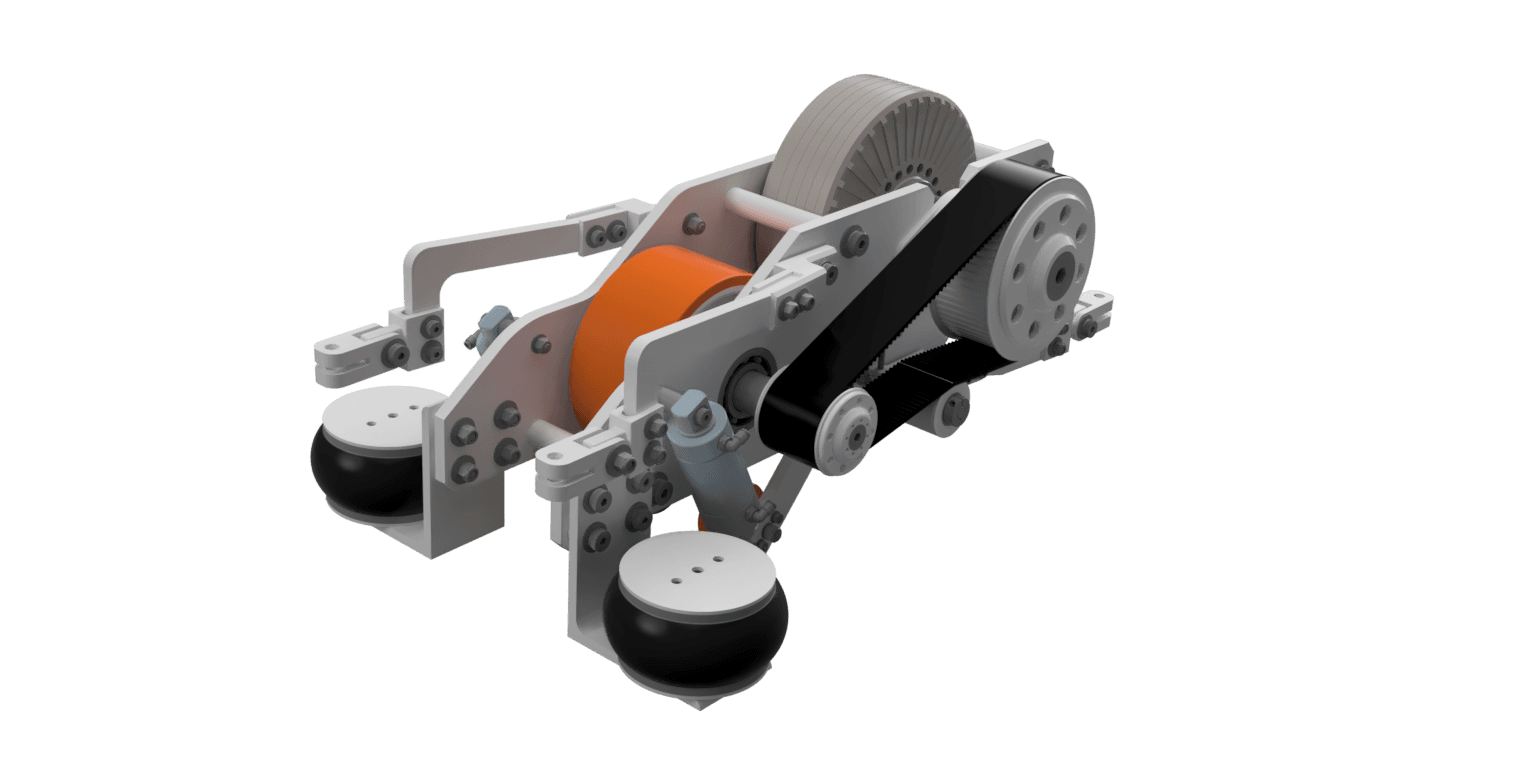
\includegraphics[width=\textwidth]{images/friction_rear.png}
\caption{Overall friction drive assembly}\label{fig:friction_rear}
\end{figure}

    \section{Structural}
    \begin{figure}
        \centering
        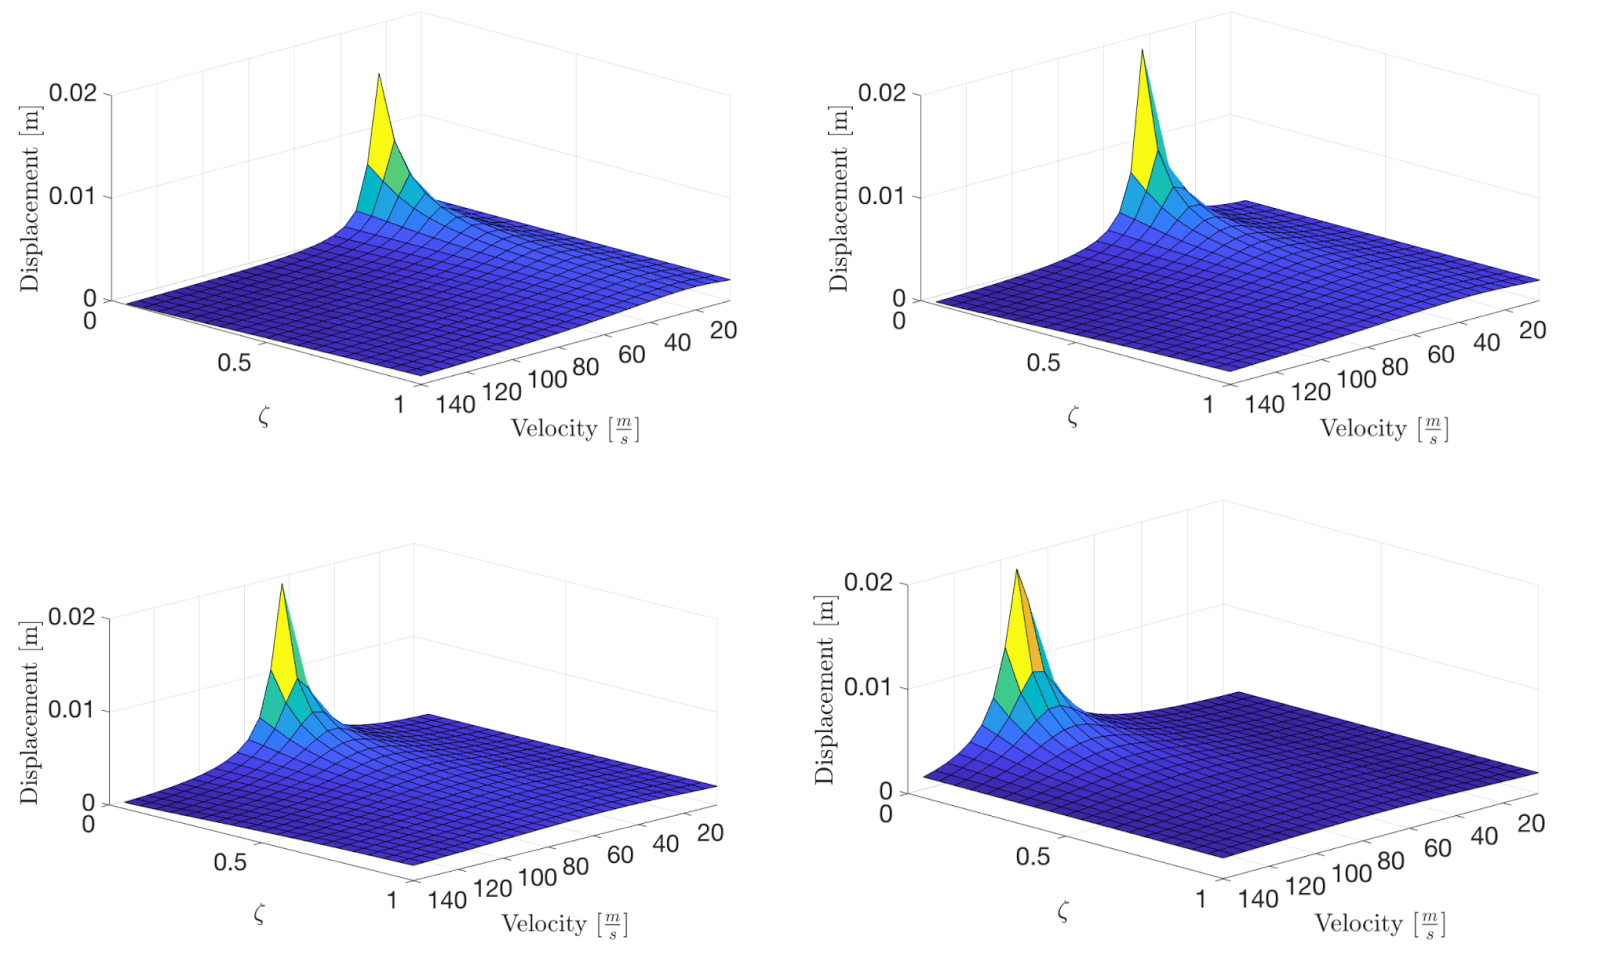
\includegraphics[width=\textwidth]{images/fig1}
        \caption{Spring constant of a. 100,000, b. 250,000, c. 500,000, and d. 1,000,000}
        \label{fig:spring1}
    \end{figure}

    \begin{figure}
        \centering
        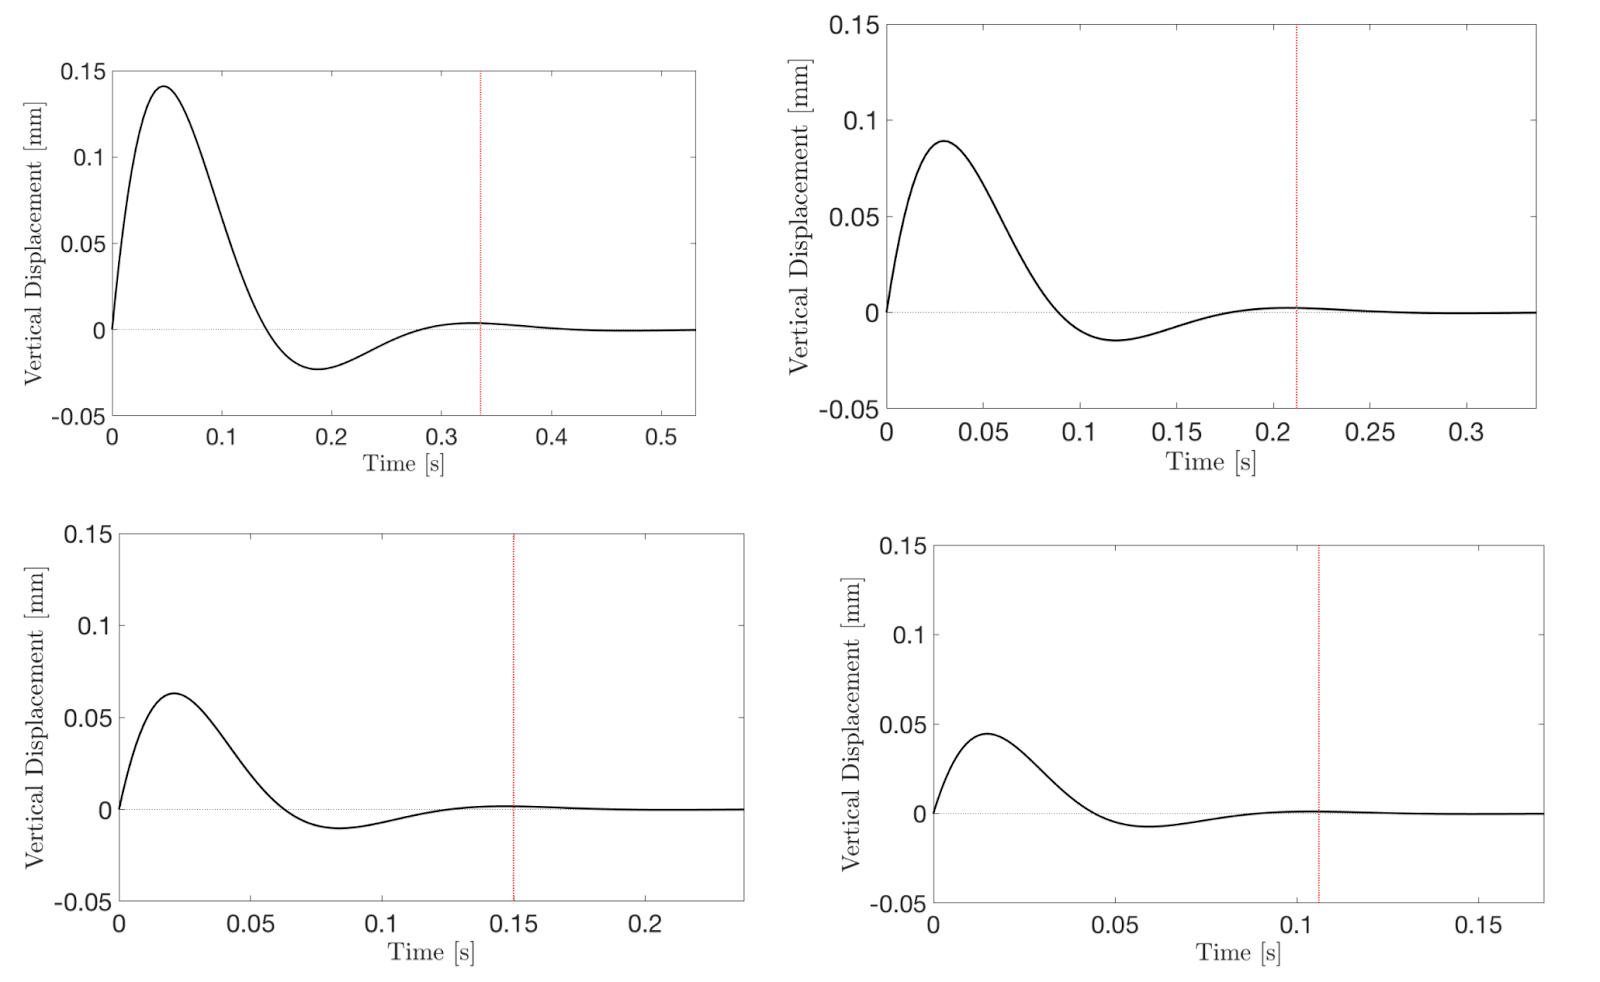
\includegraphics[width=\textwidth]{images/fig2}
        \caption{Spring constant of a. 100,000, b. 250,000, c. 500,000, and d. 1,000,000}
        \label{fig:spring2}
    \end{figure}
    In order to simulate how the pod will react to imperfections in the track, we performed two separate vibrational analyses, in the vertical and horizontal directions, with two separate vibrational damping systems (\reffig{fig:spring1} and \reffig{fig:spring2}). Based on the construction of the track, the horizontal direction will likely be by far the most problematic; this analysis is detailed in the lateral subsystem. The vertical damping system is closely integrated into the friction drive system, and so is described here.\\

    To determine design parameters of the springs and dampers, several simulations were performed. Different spring constants were chosen, and simulations for each were created using MatLab. The simulated pod was excited with a sinusoidal displacement, with amplitude as the maximum I-beam height tolerance and frequency matching the rate of I-beams passing by the pod. The magnitude of the maximum resulting pod displacement from the beam was plotted for each value of damping coefficient and speed (\ref{fig:spring1}). This series of plots shows the most dangerous combinations of damping coefficient and velocity. For each value of the spring coefficient, as the damping is increased, the vibrations become less intense. It was decided that a value of damping coefficient between [0.5 - 1.0] would be optimal in order to reduce pod vibrations.  Moving forward with this analysis, the response of the pod to a sudden displacement step was measured for a damping coefficient of 0.5 with varying spring constants. This is shown in \ref{fig:spring2}. It can be seen that as the spring coefficient is increased, the pod returns to the initial position much faster, which is shown by the red line. Also, as the spring coefficient is increased, the maximum displacement also decreases. Therefore, it was decided that the spring coefficient and damping coefficient should have values of \SI{500000}{N/m} and 0.5, respectively. \\

\begin{figure}[H]
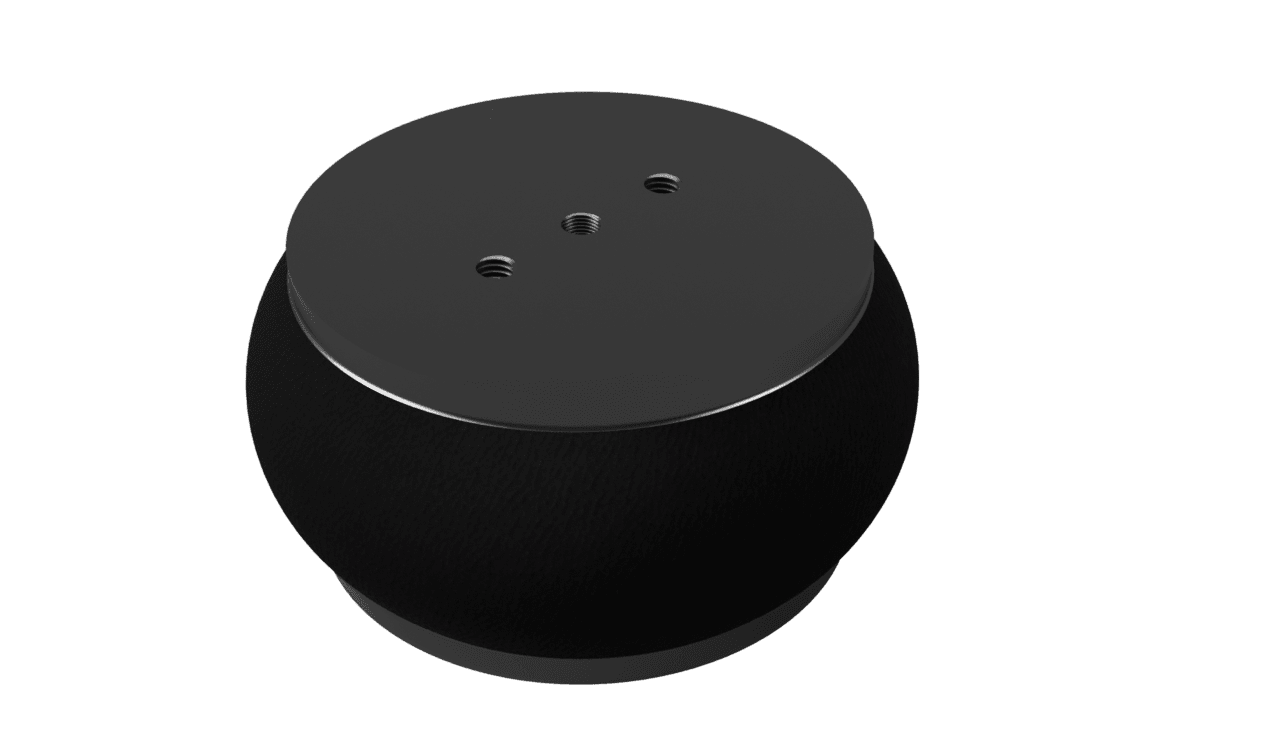
\includegraphics[width=\textwidth]{images/fig3}
\caption{CAD of air bag suspension}\label{fig:cad-air-bag}
\end{figure}

    The structure of the friction drive is designed to connect the various parts of the drive together and links it all to the frame. The main members of the structure are two vertical aluminum plates onto which all other parts are mounted. The plates are connected with four internally threaded aluminum rods. L-brackets are bolted to the front of the plates which give a horizontal surface for the airbag suspension system to rest upon. The motor is bolted to the right side plate, and the motor shaft is supported by a pillow block bearing bolted on the left plate. A Watts linkage was chosen to connect the friction drive to the frame, as it allows vertical freedom while restricting longitudinal and lateral movement in relation to the frame. The linkage is made up of four angled arms into which oil-embedded bushings are press fit to allow them to pivot about a bolt. Aluminum 6061 T6 was the chosen alloy for the structure, as it has a relatively high yield strength of 276 MPa \footnote{\url{http://asm.matweb.com/search/SpecificMaterial.asp?bassnum=ma6061t6}} and its easy machinability. The side and top views of a simplified friction drive model are shown in \autoref{fig:oll} and \autoref{fig:otl}.

\begin{figure}[H]
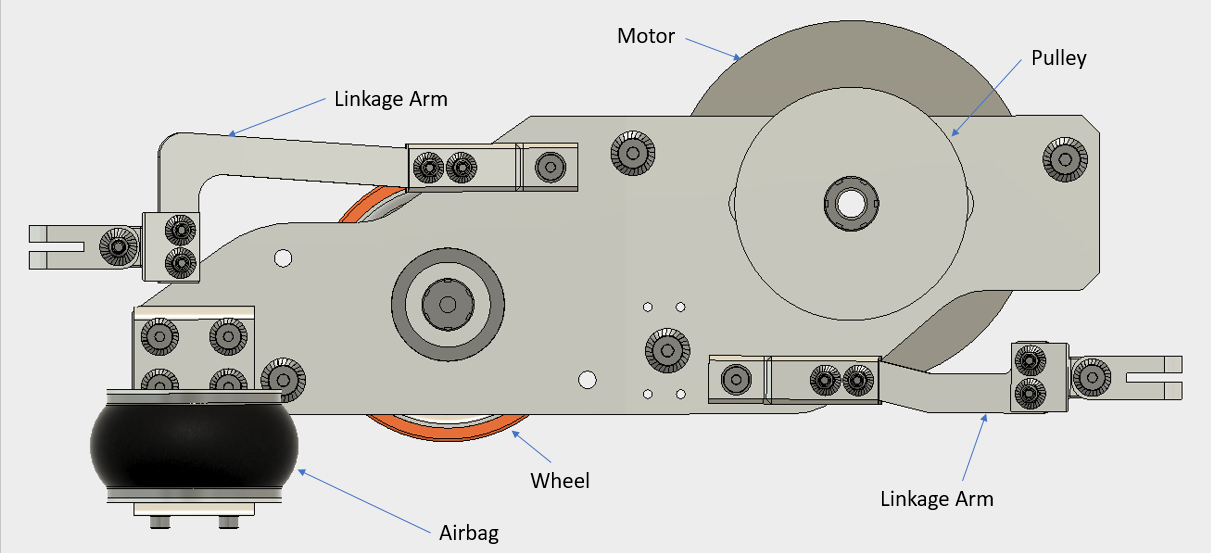
\includegraphics[width=\textwidth]{images/OrthoLeftLabelled.png}
\caption{Left side view of the simplified friction drive structure.}\label{fig:oll}
\end{figure}

\begin{figure}[H]
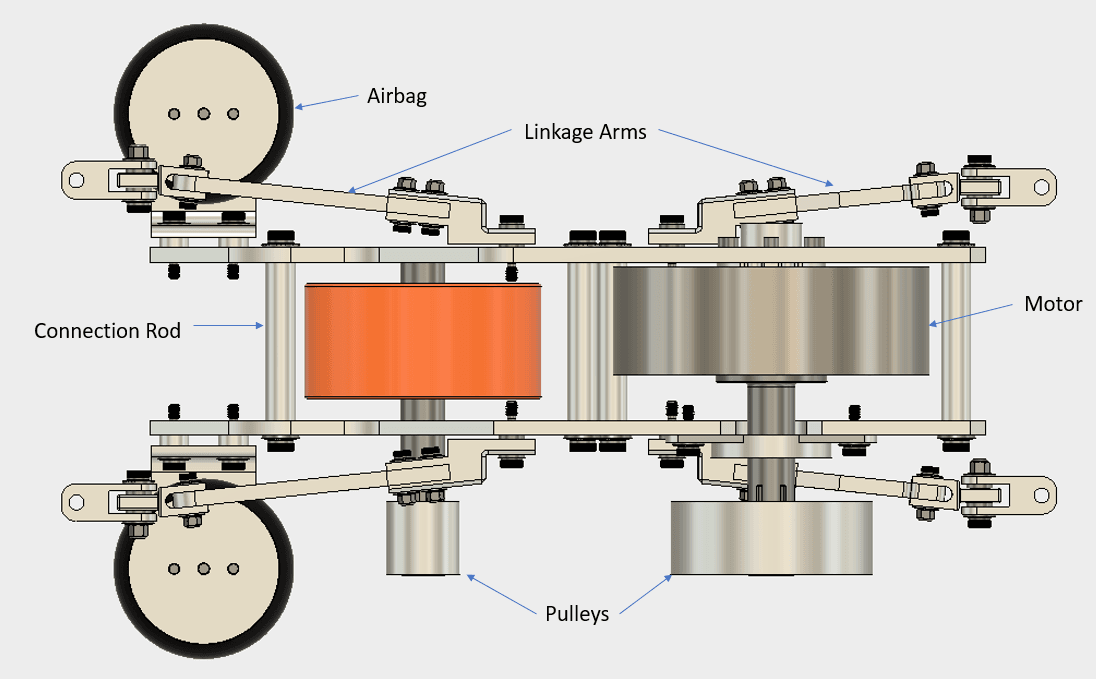
\includegraphics[width=\textwidth]{images/OrthoTopLabelled.png}
\caption{Top view of the simplified friction drive structure.}\label{fig:otl}
\end{figure}

Three test cases were chosen for the finite element analysis of the friction drive structure. Two of the cases, acceleration and braking, were normal operation loading cases, while the lateral case was an edge case load. The analysis was done on ANSYS using imported models from Fusion 360. Bolts and nuts were unthreaded, and detail was removed. All contacts were frictional with a coefficient of static friction of 1.05 \footnote{\url{https://www.engineeringtoolbox.com/friction-coefficients-d_778.html}} corresponding to that of aluminum-aluminum contact, with the exception of press-fit parts, which had bonded contacts, and the oil-embedded bushings, which had a frictionless contact. A two step analysis was performed with the first step containing all the bolt pretensions and the second step containing the loadings. The pretension loading values were calculated to be a value which would either keep the bolt's factor of safety (FOS) over 2 or the part's FOS over 3, whichever one was lower was selected. One special case is the bolts which go through the oil-embedded bushings, which had to stay under half the bushing's axial load rating. For the M8 screws going through the motor, 5500 N was chosen, while other bolts had a clamping force of 6000 N. The bolts going through the bushings were pretensioned to 2250 N. The wheel was restricted to zero displacement in the vertical direction, and the frame connection points were limited in the longitudinal and lateral directions. Other forces included the force of the belt tension on the face of the pullies, the clamping force of the track clamps on their mounting holes, and the weight of the pod on the L-brackets.\\

In the acceleration case, an additional global acceleration of 8 m/s rearwards was added to simulate a phantom force created by the non-intertial frame of reference. A forwards force of 1500 N was added to the wheel. The solve gave a maximum stress of 119.7 MPa on a motor mounting screw and an overall minimum safety factor of 2.68 which occured on an oil-embedded bushing. The max stress region is shown in \autoref{fig:accelstress}. A maximum displacement of 1.3 mm was caused on the airbag support L-bracket, shown in \autoref{fig:acceldisp}.

\begin{figure}[H]
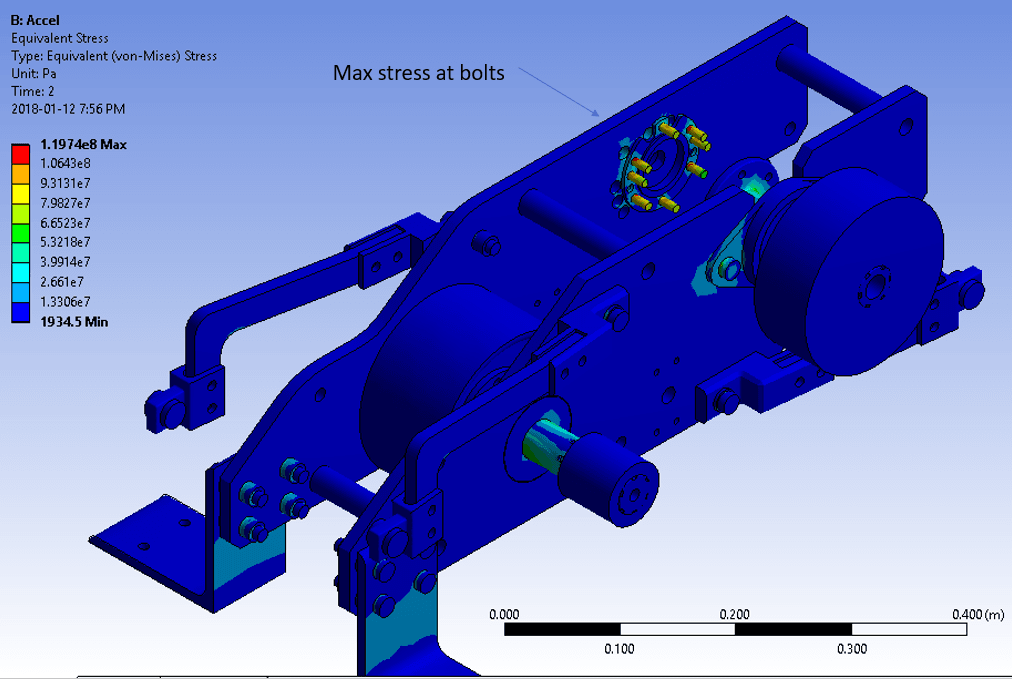
\includegraphics[width=\textwidth]{images/AccelStressLabelled.png}
\caption{Stresses on the friction drive structure during acceleration.}\label{fig:accelstress}
\end{figure}

\begin{figure}[H]
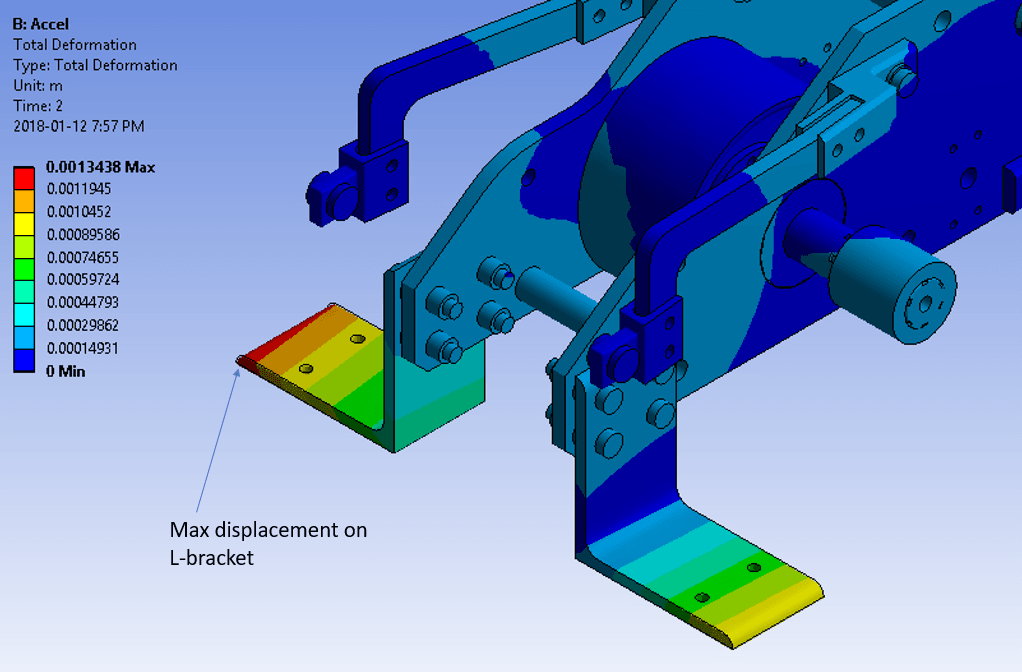
\includegraphics[width=\textwidth]{images/AccelDispLabelled.png}
\caption{Displacements on the friction drive structure during acceleration.}\label{fig:acceldisp}
\end{figure}

In the braking case, a global acceleration of 30 m/s forwards was added, as well as a cumulative force of 1500 N on the frame connections. In this case, the wheel was fixed and the frame connections unfixed in the longitudinal direction. The solve gave a maximum stress of 113.4MPa on a motor mounting screw and a minimum safety factor of 2.70. The region of greatest stress is shown in \ref{fig:brakestress}. A maximum displacement of 1.2 mm was found in the same location as the previous case.

\begin{figure}[H]
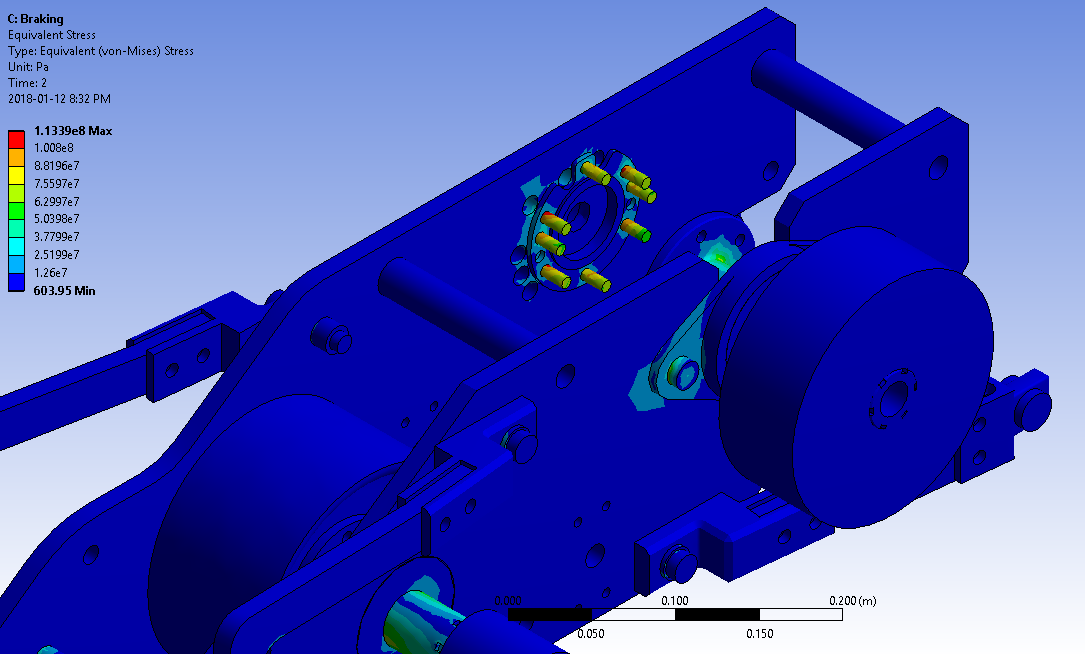
\includegraphics[width=\textwidth]{images/BrakingStress.png}
\caption{Stresses on the friction drive structure during braking. The motor is hidden for clarity.}\label{fig:brakestress}
\end{figure}

In the lateral load case, a global acceleration of 10 m/s laterally was added. The wheel was fixed in the vertical direction, and the frame contact points were fixed in the three longitudinal directions. The solve gave a maximum stress of 123 MPa on a motor mounting screw and a minimum safety factor of 2.61. A maximum displacement of 1.5 mm was generated. 

\begin{figure}[H]
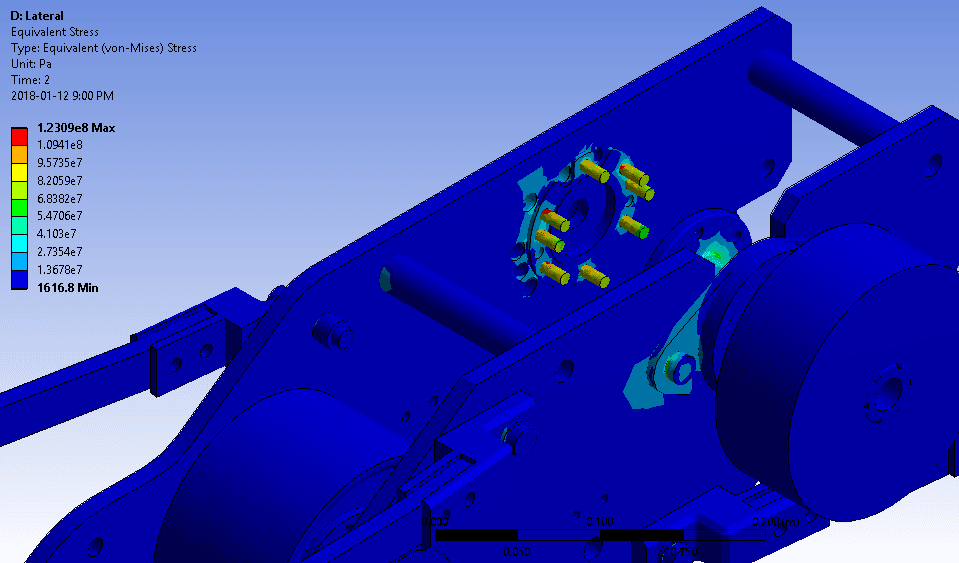
\includegraphics[width=\textwidth]{images/LateralStress.png}
\caption{Stresses on the friction drive structure during the lateral edge case. The motor is hidden for clarity.}\label{fig:latstress}
\end{figure}

    \section{Motor}
    A number of different types of electric motors were investigated to select one that was best suited for our applications, primarily AC induction motors and DC brushless motors. Specifically, axial flux motors were favoured due to their high power density and efficiency. These motors are very light and can provide high torque and power with low heat loss.\\

    It came to several choices of motors from electric motor manufacturers, YASA and EMRAX, that specialize in producing commercial axial flux motors. Several product criteria that affected this choice included:
    \begin{itemize}
        \item Specific power density
        \item RPM range
        \item Torque and power profiles
        \item Efficiency/thermal generation
        \item Mass
        \item Power consumption
        \item Cost
    \end{itemize}

    Based on these criteria, the EMRAX 268 was chosen.\\

    \begin{figure}
        \centering
        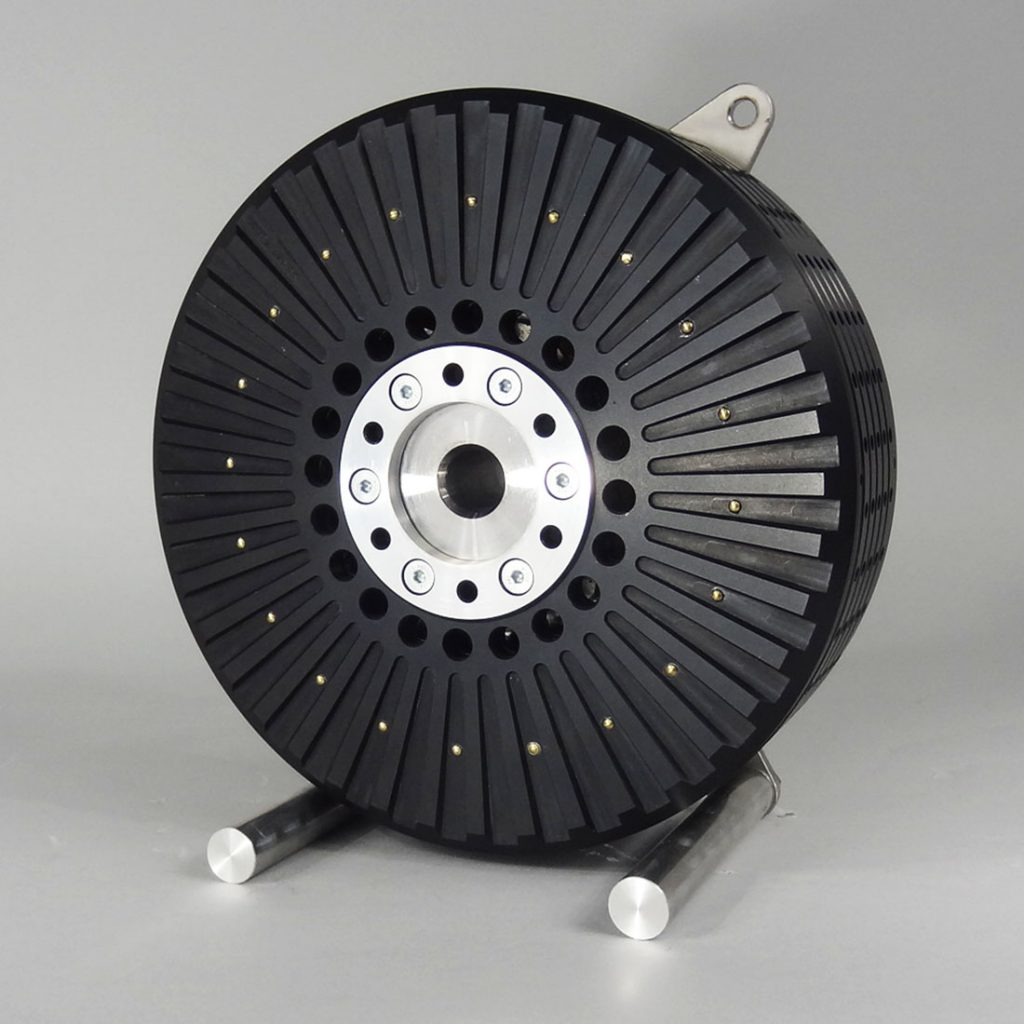
\includegraphics[width=0.5\textwidth]{images/fig4}
        \caption{Side profile of EMRAX 268 Axial Flux Electric Motor}
        \label{fig:emrax-profile}
    \end{figure}
    \begin{figure}
        \centering
        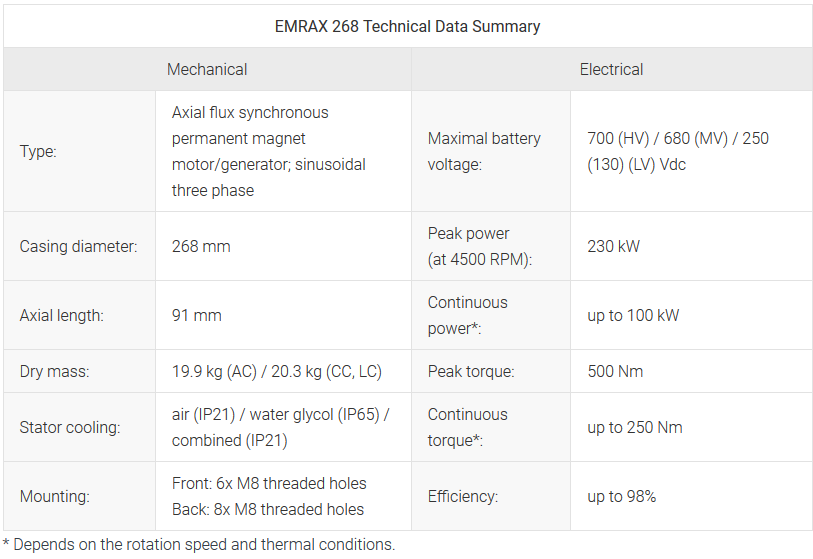
\includegraphics[width=\textwidth]{images/fig5}
        \caption{Summary of EMRAX 268 Motor Technical Specifications \protect\footnote{https://paperpile.com/c/T85mA9/hmBQ}}
        \label{tab:emrax-specs}
    \end{figure}

    \begin{figure}
        \centering
        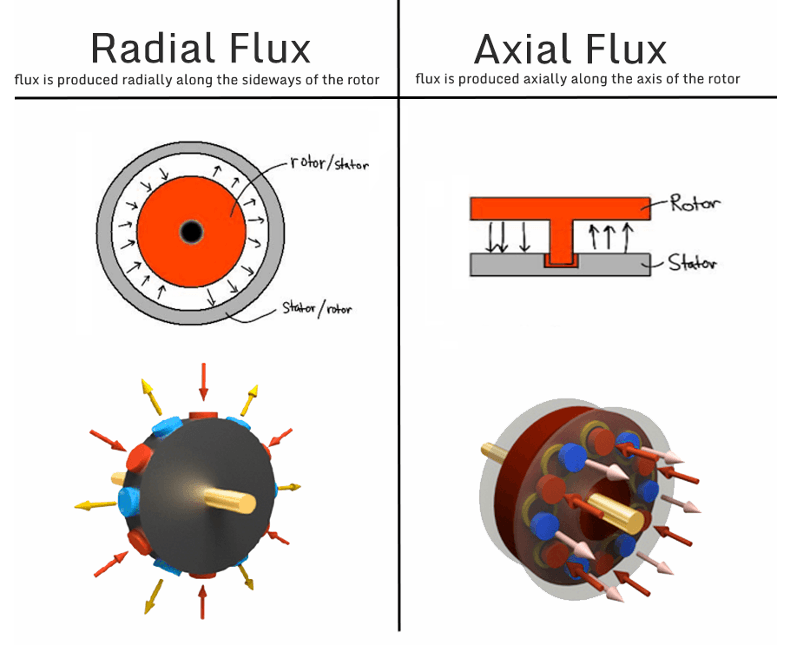
\includegraphics[width=\textwidth]{images/fig6}
        \caption{Axial Flux Motors are built in the same fashion that regular permanent magnet motors are. However, the positions of the stator and rotors are reversed, where the outer casing is the rotor and the inner core is the stator. In addition, most electric motors are radial flux motors where the magnetic flux is oriented along the radial of the stator. Axial flux, as said in the name, orient their magnetic flux axially around the axis of the rotor\protect\footnote{\url{https://paperpile.com/c/T85mA9/rsJD}}.}
        \label{fig:axial-vs-radial}
    \end{figure}
    \begin{figure}
        \centering
        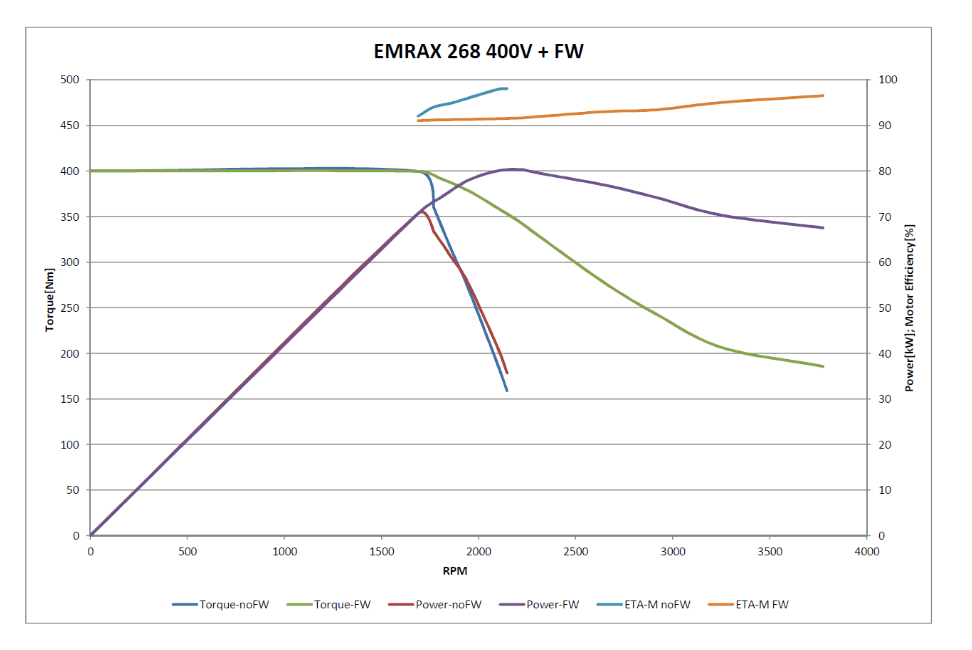
\includegraphics[width=\textwidth]{images/fig7}
        \caption{EMRAX 268 Torque, Mechanical Power, and Efficiency curve over RPM\protect\footnote{\url{https://paperpile.com/c/T85mA9/vP1A}}}
        \label{fig:emrax-efficiency}
    \end{figure}
    \subsection{Motor Performance}
    The graph in \reffig{fig:emrax-efficiency} shows the torque, power and efficiency of the motor over RPM. As mentioned previously, the motor is capable of instantaneously producing a peak torque of \SI{400}{Nm}. EMRAX states that the motor is capable of greater RPM ranges by utilizing MFW (magnetic field weakening). The effect of MFW is significant in reducing the decay of torque at higher RPM ranges, and producing higher mechanical power. This is accomplished by reducing the overall efficiency of the motor. However, the reduction is not significant (\textless8\% greater loss), and the gains in performance outweigh the loss in efficiency.\\

    \begin{figure}[H]
        \centering
        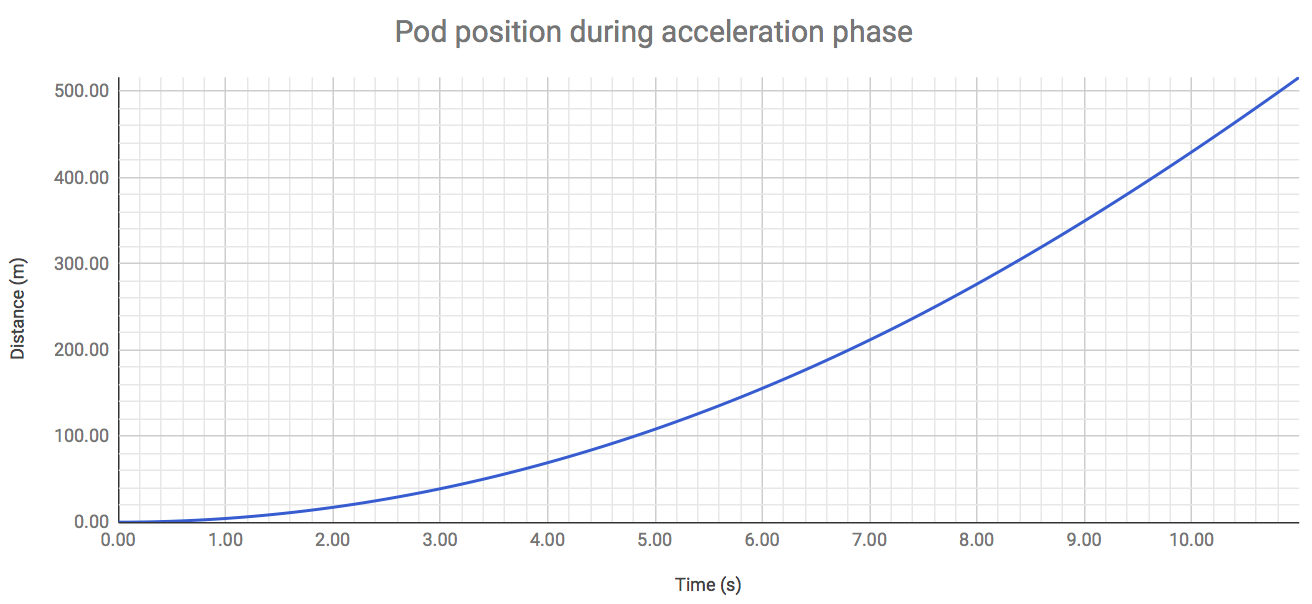
\includegraphics[width=\linewidth]{images/pod_position_vs_time_curve.png}
        \caption{Pod position during acceleration phase}\label{pod-position}
    \end{figure}
    
    \begin{figure}[H]
        \centering
        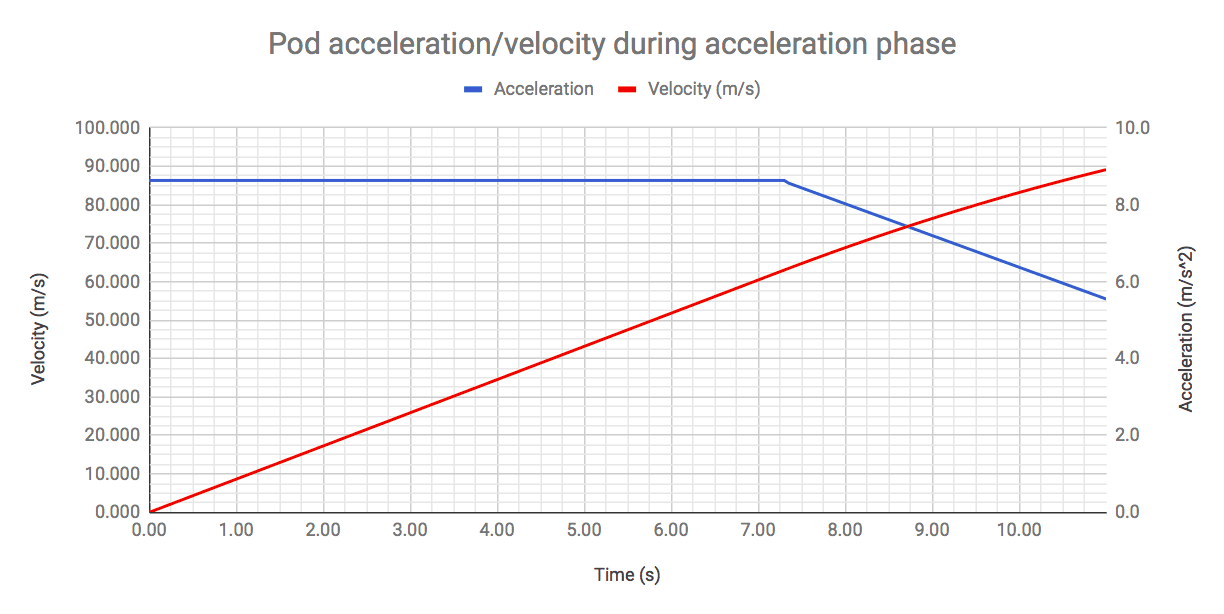
\includegraphics[width=\linewidth]{images/pod_acceleration_velocity_vs_time_curve}
        \caption{Pod acceleration/velocity during acceleration phase}
    \end{figure}
    \begin{figure}[H]
        \centering
        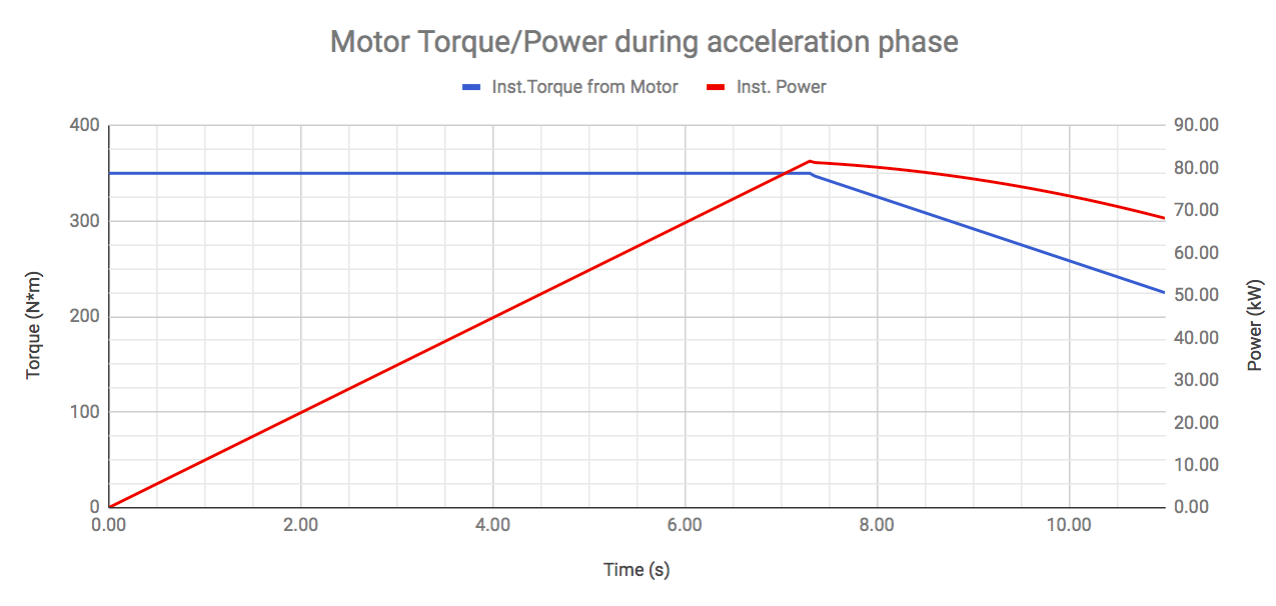
\includegraphics[width=\linewidth]{images/torque_power_vs_time_curve}
        \caption{Motor Torque/Power during acceleration phase}
    \end{figure}
    \begin{figure}[H]
        \centering
        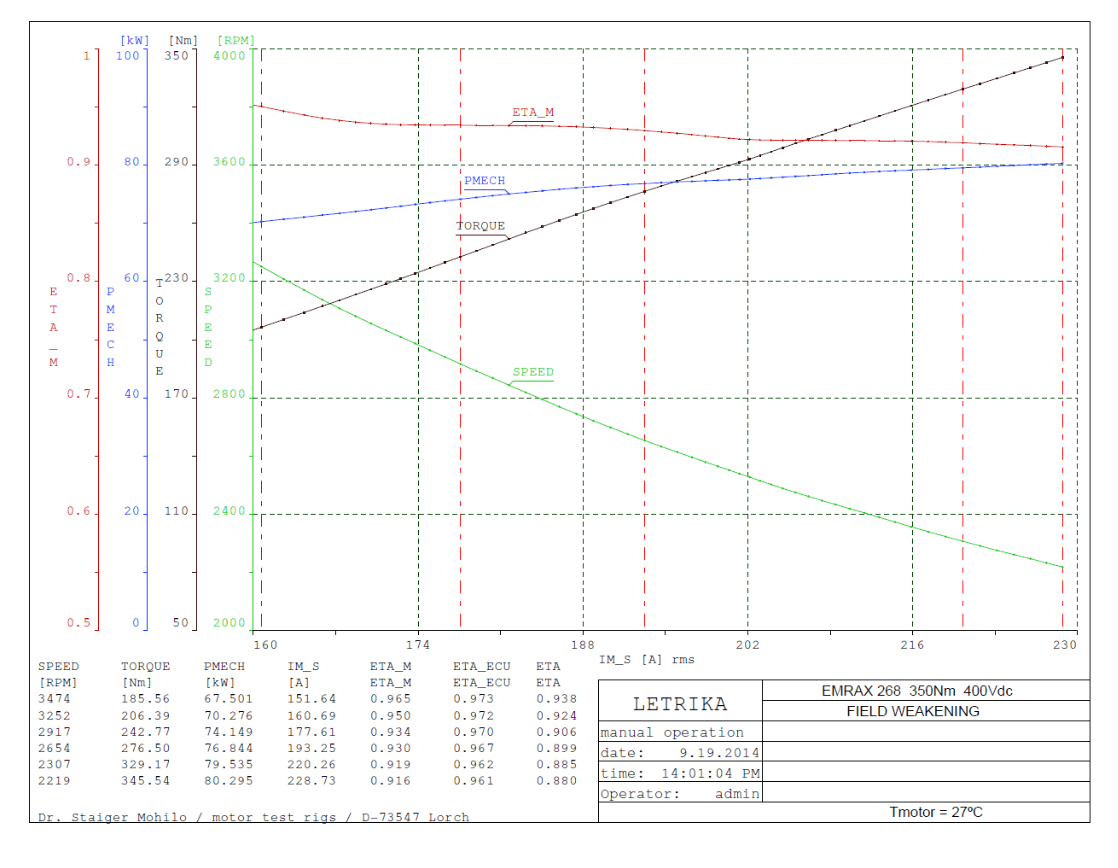
\includegraphics[width=\linewidth]{images/fig11}
        \caption{EMRAX 268 Motor Specifications\protect\footnote{\url{http://emrax.com/wp-content/uploads/2017/01/emrax_268_technical_data_4.5.pdf}}}
    \end{figure}

    \section{Power Delivery}
    The EMRAX 268 has a variety of shaft mounting solutions. The most practiced ones are bolted flange shafts or a shaft within the splined hub of the motor. The flanged shaft was the choice for the design because of the ease at which one can assemble and perform maintenance on the powertrain and the versatility to alter shaft lengths and dimensions. In addition, in order to secure pulleys onto this shaft, the option of splining a shaft is available, which provides the most secure and efficient method of doing so. The shaft is made out of hardened steel (42CrMo4QT) which is commonly used to make driveshafts, turbocharger gears, and crankshafts.\\

    \begin{figure}[H]
        \centering
        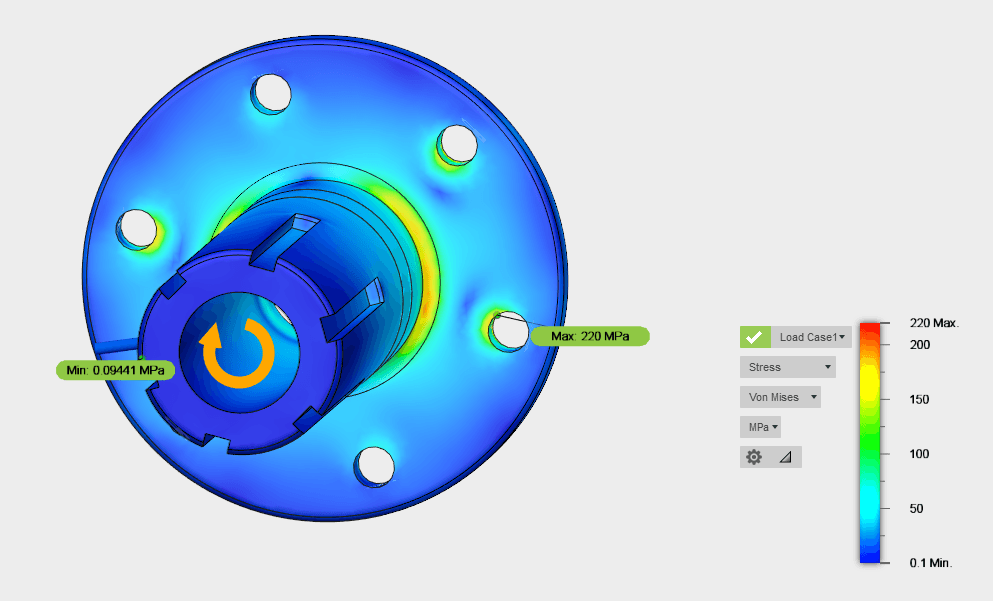
\includegraphics[width=\linewidth]{images/fig12}
        \caption{Stress Analysis on motor shaft}
    \end{figure}
    \subsection{Motor Shaft}

    Static stress FEA was performed in Autodesk Fusion 360 on the shaft in order to analyze stress concentrations and possible failures. The shaft was fixed via the bolt holes within the flange and the load was equivalent to the tension force that the pulley and belt system would exhibit at peak loads. In addition, an angular load was placed onto the shaft, equivalent to the maximum possible RPM range the motor could produce, which is equivalent to \SI{575}{rad/s}.\\

    The shaft experiences a peak stress of \SI{220}{MPa}, located at the bolt holes on the flange. This raises concern regarding bolts that fasten the shaft to the motor. Reaction force was measured to be a peak of around \SI{400}{N} on the bolt, which means based on the cross sectional area of the bolt, shear force and moment, it would experience a peak of \SI{338}{MPa}. This is within the yield strength of the bolt which is less than \SI{965}{MPa} yield strength, resulting in a safety factor of approximately 3.\\

    \begin{figure}
        \centering
        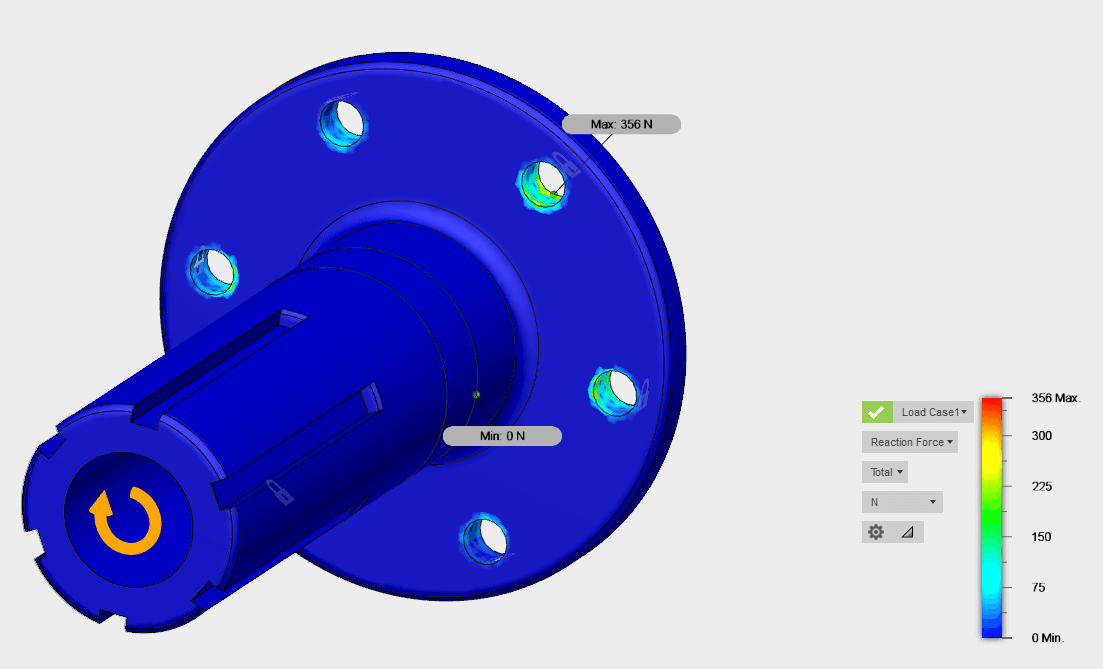
\includegraphics[width=\linewidth]{images/fig13}
        \caption{Reaction force of bolted motor shaft}
    \end{figure}
    \begin{figure}[H]
        \centering
        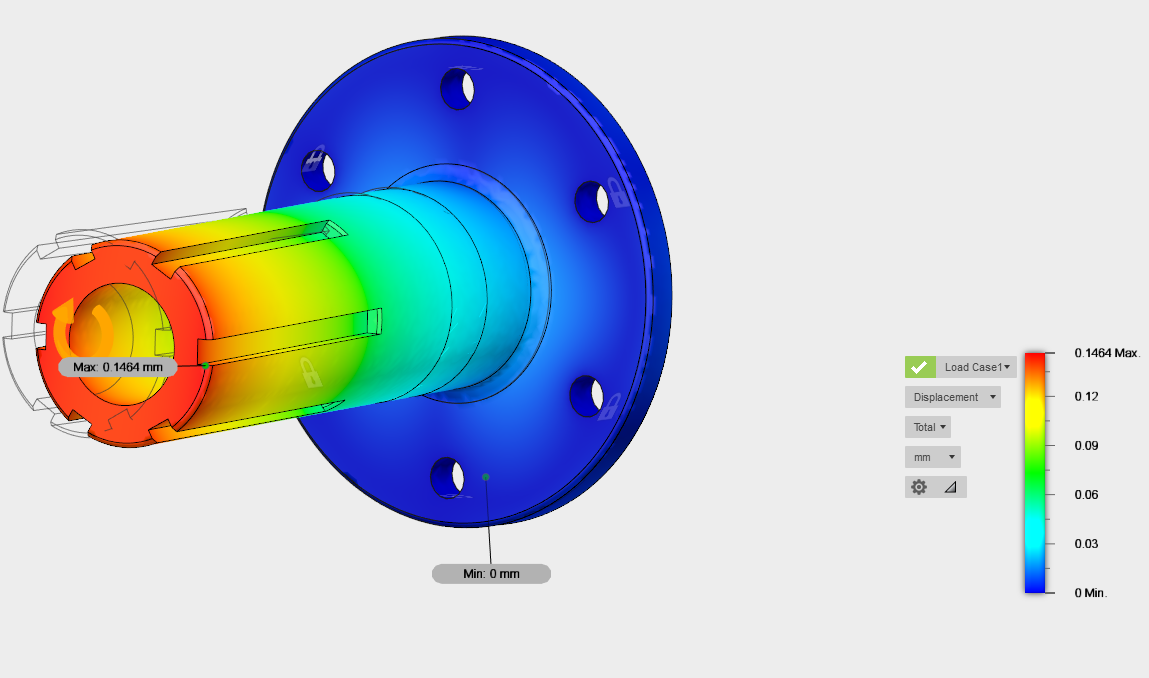
\includegraphics[width=\linewidth]{images/fig14}
        \caption{Displacement of Shaft FEA}
        \label{fig:shaft-stress1}
    \end{figure}

\ref{fig:shaft-stress1} shows the displacement result of the FEA, where the peak displacement of the shaft is \SI{0.15}{mm} at the tip of the shaft. In the image shown, it is at a 5\% model based displacement adjustment. The mesh was created with an average element size of 3\% of the model based size had a parabolic element order. To refine our mesh and create more accurate results, adaptive mesh refinement was done in the areas of peak stress, at a cycle of 3 mesh refinements with a convergence tolerance of 5\%. Similar FEA was done on the other power transmission shaft that connects to the wheel. The result yielded less overall stress on the bolt holes due the shaft not having a hollowed core (\SI{220}{MPa}).\\

    \begin{figure}[H]
        \centering
        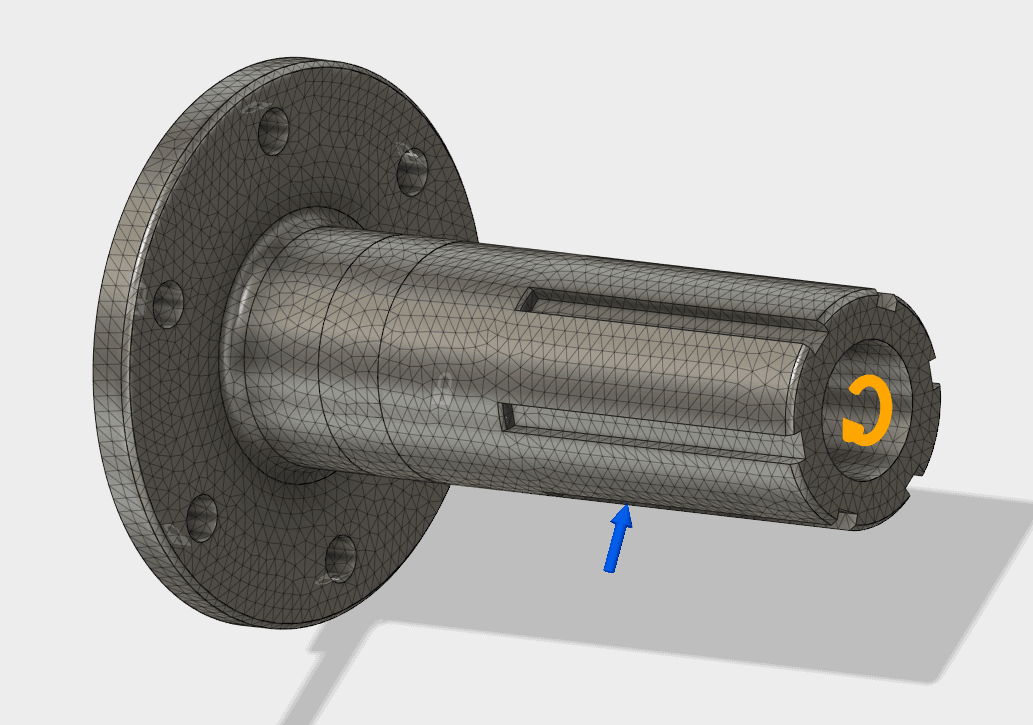
\includegraphics[width=\linewidth]{images/fig15}
        \caption{Meshing of the Shaft FEA}
    \end{figure}
    The mesh was created with an average element size of 3\%  of the model based size had a parabolic element order. To refine our mesh and create more accurate results, adaptive mesh refinement was done in the areas of peak stress, at a cycle of 4 mesh refinements with a convergence tolerance of 5\%.

    \subsection{Pulley and Belt Drive}
The propulsion system utilizes a single gear reduction in an open belt system, that incorporates an idler pulley to maintain constant tension on the system. Many different power transmission options were investigated, including a multi-gear system and a continuously variable transmission (CVT) system. However, these options were not chosen due to the overall complexity that these systems would have, and the cost, research, and development time involved in developing these systems would be far beyond the timeline allocated for the competition. Thus, a single gear reduction with the open belt system was chosen for the simplicity of design and testing, and the reduction of overall costs to integrate this power transmission system onto the pod.\\
\begin{figure}[H]
            \centering
    \begin{subfigure}{0.5\textwidth}
        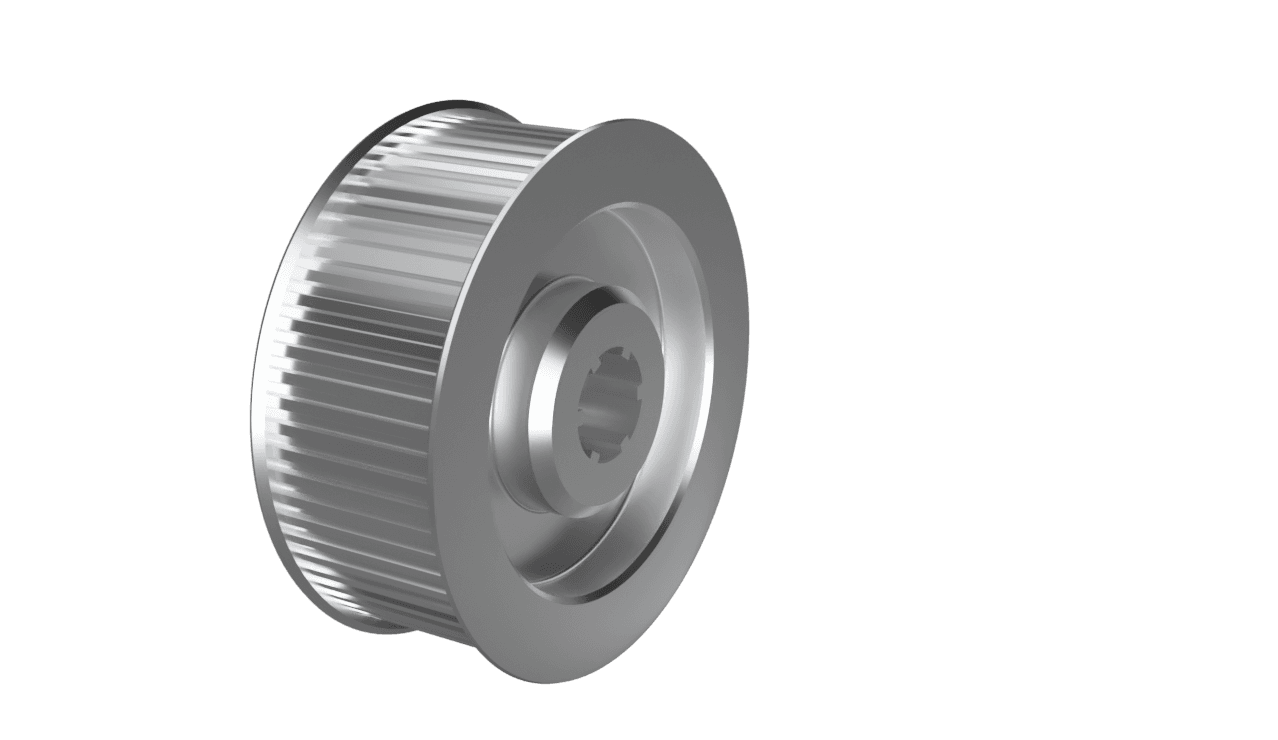
\includegraphics[width=\linewidth]{images/fig16}
        \caption{Timing belt pulley}
        \end{subfigure}

        \begin{subfigure}{0.25\textwidth}
        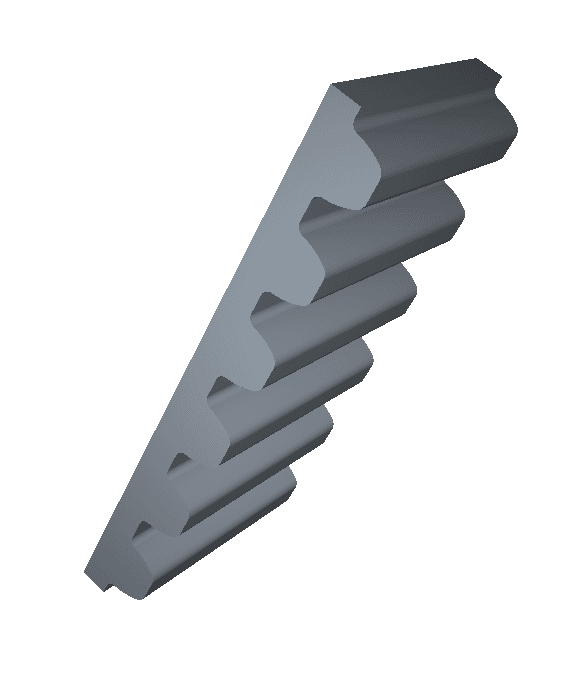
\includegraphics[width=\linewidth]{images/belt.png}
        \caption{Section of a synchronous belt}
        \end{subfigure}
        \caption{Pulley and Belt Drive}
        \label{fig:pulley}
\end{figure}

Two of the most common open belt configurations that exist are V-belts and synchronous or timing belts. The V-belt is a smooth belt, and relies on the friction between itself and the pulleys to transfer forces. It a cross-section shaped like a V, which runs through pulleys with a groove. This shape gives a V-belt a much higher coefficient of friction than a regular flat belt, and thus it can transfer more power. The other belt option to consider was a timing belt. It consists of a flat belt with small ridges lining the inner surface. The pulleys, called sprockets, have notches in which the belt's ridges fit. The ridges eliminate the reliance on friction, and unlike a friction belt it will not slip under high loads unless the belt fails mechanically.

After consulting GATES, a reputable corporation that manufactures power transmission components, it was recommended that a timing belt be used based on the high power and high angular velocity of the motor. Another advantage of timing belts is that they have a smaller minimum bend diameter due to their flat cross-section. This is significant since the pulleys' sizes are restricted by the friction drive and frame design. The driving and driven pulleys had to be small enough to fit, but large enough to exceed the minimum bend diameter of the belt. Lastly, timing belts are generally able to handle more power than friction belts.

Both of the pulleys are to be made out of AL 6061-T6511; chosen because of the high yield strength and low density that 6061-T6 possesses while being a cost-effective solution. The pulleys will both be splined onto the shaft to ensure that the pulley does not slip on the shaft while transferring power. In addition, the pulley face itself will be slotted along the outside to fit a synchronous belt (timing belt) of the GATES Poly Chain GT Carbon series, which was recommended to us by the manufacturer.

GATES recommends a minimum of 22 teeth for a sprocket\footnote{``Preventative Maintenance and Safety Manual - GATES Corp.''\url{https://safety.gates.com/wp-content/uploads/2016/04/Gates-Corporation-Preventive-Maintenance-Safety-for-Belt-Drives-Guide.pdf}}.
\begin{equation}
C = \pi d \textrm{ and } C=\frac{\textrm{number of teeth}}{P}
\end{equation}
Rearranging, the following is obtained:
\begin{equation}
\textrm{number of teeth}=\frac{\pi d}{P}
\end{equation}
With a belt pitch $P$ of \SI{8}{mm}, and a diameter $d$ of approximately \SI{62}{mm}, the smaller pulley would have:
\begin{equation}
\textrm{number of teeth}=\frac{\pi \times \SI{62}{mm}}{\SI{8}{mm}}\approx 24
\end{equation}
Note that the actual diameter of the pulley would have to be slightly more than \SI{61}{mm} in this case, to let the number of teeth be a whole number.
This meets GATES' recommended pulley size in order to maximize belt efficiency, safety and lifespan.

Power will be transferred from one pulley to the other by the aforementioned GATES belt. The Poly Chain GT Carbon belt is a synchronous belt (timing belt) that satisfies the motor's high torque and power output, while reducing the requirement for a large thick belt and a high tension. These belts have a mechanical efficiency that can exceed 97\% when the belt is in well-maintained condition. It was chosen by consulting GATES about the pod's design requirements and through use of GATES's Design Flex Pro, an application that outputs a list of power transmission design solutions based on the expected RPM ranges, speed ratio and input loads. The belt is predicted to experience peak tension forces of approximately \SI{4500}{N}. The belt’s ultimate tensile strength is rated to handle \SI{22700}{N} per inch of belt width. Since the chosen belt for the friction drive is around \SI{2.5}{in} wide, the belt is more than capable of handling its tensile loads.

Using the expected pod mass and the motor's specifications, the pod is projected to reach speeds in excess of \SI{88}{m/s}.\\

	\begin{figure}
        \centering
        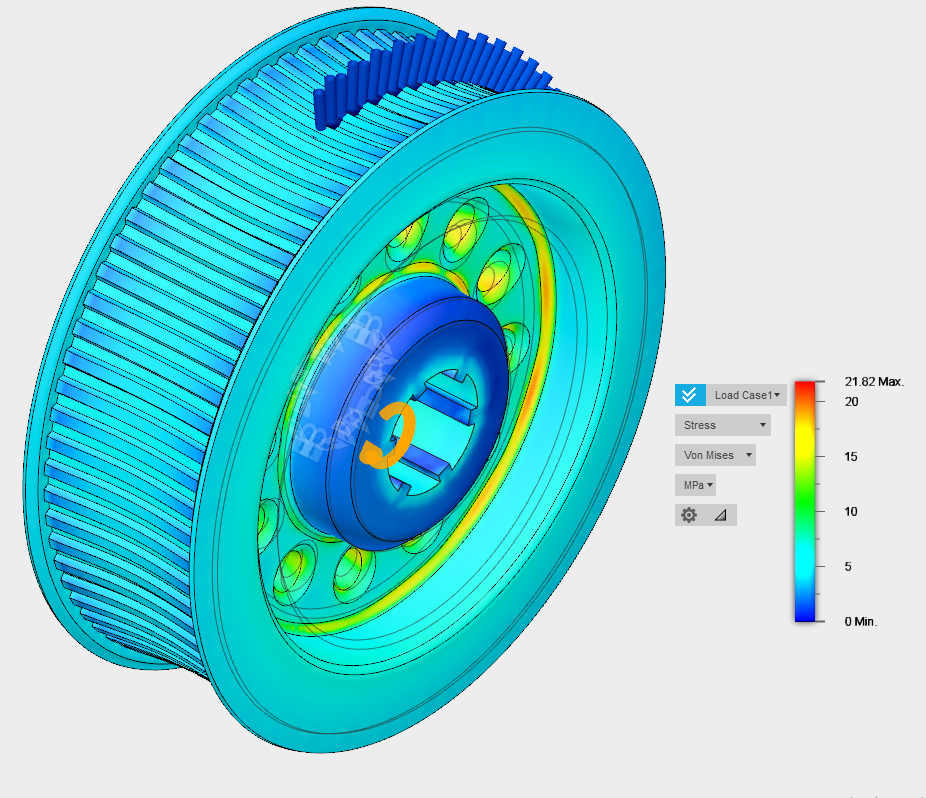
\includegraphics[width=0.75\linewidth]{images/pulley}
        \caption{Large pulley FEA results}
        \label{fig:pulley2}
    \end{figure}

    Static stress FEA, completed using Autodesk Fusion 360 software, assured us that the pulley will be able to withstand the peak compressive forces from the belt tension (\SI{4500}{N}) and the calculated RPM ranges for the drive pulley (0-\SI{3000}{RPM}). The pulley, made out of Aluminum 6061-T6, has a yield strength of \SI{275}{MPa}. The peak stress experienced by the drive pulley is about \SI{22}{MPa}, which is significantly lower than the material’s yield strength. This high safety factor is necessary due to the fatigue cycles that the pulley will experience. The fatigue strength of 6061-T6 is about \SI{96}{MPa} after $5\times 10^8$ cycles\footnote{``Aluminum 6061-T6 - ASM Material Data Sheet - MatWeb.'' \url{http://asm.matweb.com/search/SpecificMaterial.asp?bassnum=ma6061t6}}. With our RPM ranges, where one whole rotation of the pulley can be considered a complete cycle going through a crest and trough of peak stress, the pulley will reach this fatigue strength after 2700 hours of running the pulley at a sustained peak RPM.\\

\begin{figure}
    \centering
    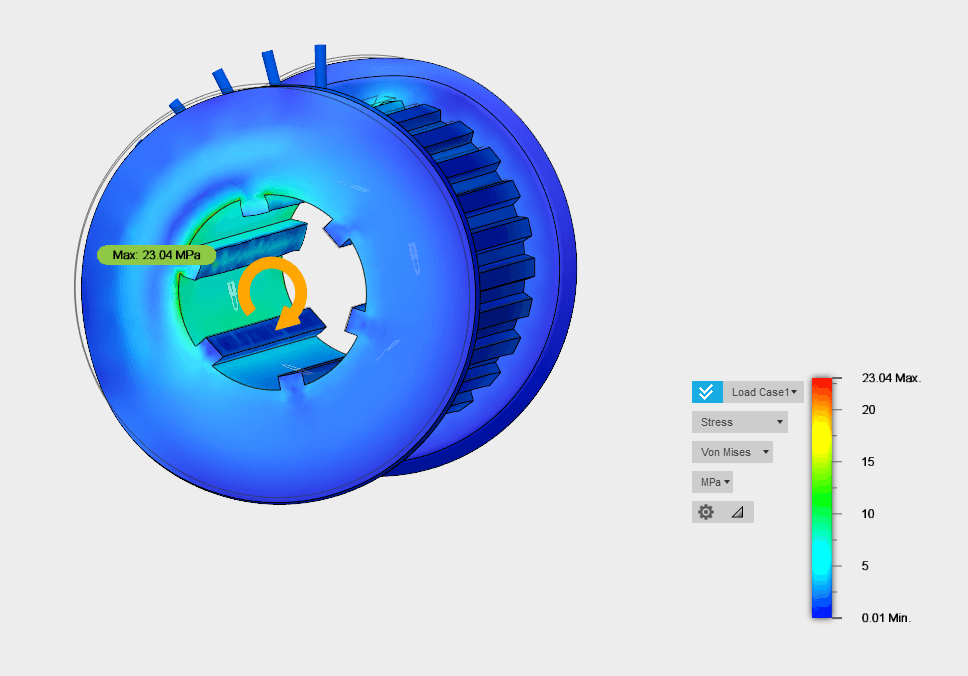
\includegraphics[width=0.75\linewidth]{images/pulley3.png}
    \caption{Small pulley FEA results}
    \label{fig:pulley3}
\end{figure}

	The driven pulley experiences the same loading characteristics as the drive pulley. Both are suitable for the loads and speeds that our design intent requires. In addition, the fatigue strength AL 6061-T6 will be sufficient for our loads and will not exhibit any failing. However, the pulleys will be replaced after 2700 hours for redundancy and safety. To reduce vibrations during high speed operation and acceleration phase, the pulleys will be produced via CNC and then two plane balanced in order to alleviate said issue.\\

	The Poly Chain GT Carbon belt is a synchronous belt (timing belt) that satisfies our high torque and power output, while reducing the requirement for a large thick belt and a high tension. The belts are have very high mechanical efficiency, with it being above 97\% when the belt is in well-maintained condition \footnote{``Timing Belt Advantages \& Disadvantages | Pfeifer Industries.'' \url{http://www.pfeiferindustries.com/timing-belt-advantages-disadvantages-i-15-l-en.html}}. This was chosen the Design Flex Pro Program provided by GATES which finds a suitable belt for a given set of operating conditions. The peak tension forces that are expected to be experienced by the belt would be 4500N. The belt’s ultimate tensile strength can handle 22700N, if assuming a belt width of an inch\footnote{Synchronous Belt Data Summary -cloudfront.net.\url{https://dpk3n3gg92jwt.cloudfront.net/domains/bbman2/trumotionsyncdata_final_3-8-07.pdf}}. Since the belt that we have specified is around \SI{2.5}{in} wide, the belt is more than capable of handling our tensile loads.\\

  \begin{figure}
    \centering
    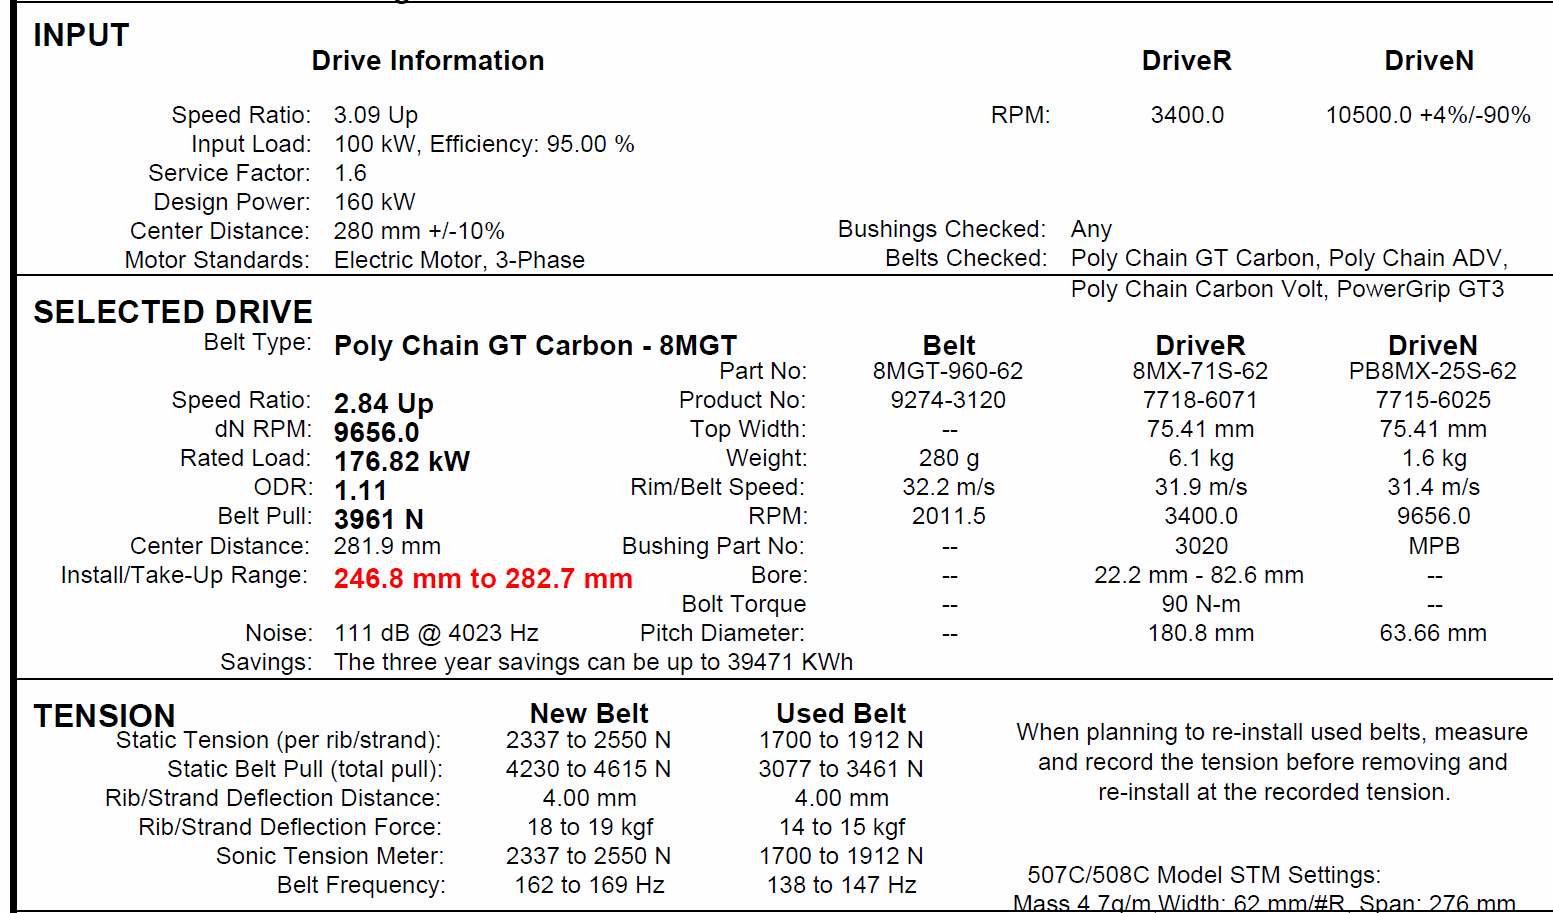
\includegraphics[width=0.75\linewidth]{images/gates.png}
    \caption{Results from GATES Design Flex Pro software}
    \label{fig:gates}
\end{figure}

\ref{fig:gates} displays the information displayed by the GATES Design Flex Pro Program when finding the appropriate belt for our design intent. All of the given requirements were based on the upper bounds of requirements of the power delivery system. It is highly unlikely that the motor will achieve the power or RPM ranges listed in the figure; however, it was required to account for redundancy and safety. The ‘Install/Take-Up Range’ is highlighted in red due to the fact that this using a pre-modeled and manufactured belt length. Since GATES is able to produce a custom belt length for our needs, this number is not of importance when determining the suitability of the belt.

Using the chosen pulley sizes, the belt length can be found.
\begin{equation}
L = 2C\sin{(\frac{\beta_r}{2})}+{\frac{1}{2}}(\beta_rR_r)+{\frac{1}{2}}(\beta_nR_n)
\end{equation}
Where $\beta$ is the angle of wrap of the belt around a pulley, $C$ is the distance between pulley centres, and $r,n$ denote driver and driven pulleys, respectively.
Using these numbers, the friction drive would require at least a \SI{778}{mm} belt.

    \subsubsection{Vacuum Compatibility}
    We have identified two potential issues with the motor in vacuum, which we have discussed with the manufacturer EMRAX.
    \begin{itemize}
        \item Cooling of the motor may be designed for air environments, where air convection plays a role in addition to the liquid cooling system.
        \begin{itemize}
            \item EMRAX believes that due to the very short runtime (less than 30 seconds) there will be no significant difference in the efficiency of the cooling system in vacuum.
            \item They have also suggested that no cooling system is needed at all, and the heat capacity of the motor itself is enough to last 30 seconds without reaching 50 degrees Celsius. We decided to design a cooling system anyway, on the grounds that it would be prudent to have and could be relatively trivially removed if physical tests show it to be significantly redundant.
        \end{itemize}
        \item Outgassing of the epoxy used to secure the motor’s internal components could weaken these fastenings and also deposit epoxy on other parts of the motor.
        \begin{itemize}
            \item EMRAX has confirmed that the motor’s internal components are both mechanically and chemically secured, so that even with epoxy outgassing there will be no problems in fastening.
            \item Deposition of epoxy could damage other parts within the motor.
        \end{itemize}
    \end{itemize}

\section{Bearings}
All bearings used in Friction Drive have been sourced to exceed the required RPM and load ranges by a large safety factor. The majority of bearings sourced are Deep Groove Bearings which are capable of high RPM ranges, with an incredibly high mechanical efficiency and low heat generation. These bearings are also capable of handling large static and dynamic loads, often exceeding \SI{5}{kN} as a standard rating. The bearings have primarily been sourced by one manufacturer to maintain consistency for dimensions, tolerance and performance. The bearings manufacturer is SKF, which specializes in high speed bearings at high axial and thrust loads. These bearings are summarized in Table \ref{table:bearingtable}.\\

\begin{table}
\centering
  \begin{tabular}{@{}l l r r l@{}} \toprule
    Part Number & Type of Bearing & Limiting Speed & Dynamic Load Rating & Location \\ \midrule
    SKF D/W R8 R-2RZ & Deep Groove Ball Bearing & 30,000 $\frac{\mathrm{rev}}{\mathrm{min}}$ & \SI{4.4}2{kN} & Guide Wheel\\
    RLS 12 & Deep Groove Ball Bearing& 11,000 $\frac{\mathrm{rev}}{\mathrm{min}}$ & \SI{30.7}{kN} & Motor Plate\\
    NKS 25 & Needle Roller & 17,000 $\frac{\mathrm{rev}}{\mathrm{min}}$ & \SI{27.5}{kN} & Front Wheel\\
    RLS 4 & Deep Groove Ball Bearing & 32,000 $\frac{\mathrm{rev}}{\mathrm{min}}$ & \SI{7.2}8{kN} & Tensioner \\
    1209 EKTN9 & Self-Aligning Ball Bearing & 11,000 $\frac{\mathrm{rev}}{\mathrm{min}}$ & \SI{22.9}{kN} & Pillow Block \\  \bottomrule
  \end{tabular}
  \caption{Bearing Specifications}
  \label{table:bearingtable}
\end{table}

    \section{ESC}
    EMRAX recommended several electronic speed controllers (ESC) and the UniTek Bamocar D3 stood out due to its low-cost and well-balanced performance. With our settings, the controller will receive an input voltage of approximately 500 V and a current of 180 A. The controller also comes with a liquid cooling system that is situated at the bottom of the controller.\\

	The ESC allows us to control the RPM to different levels. Since RPM is related to power and torque according to the following equation, it'll aid in maintaining a constant desired torque value of \SI{350}{Nm}.

     \begin{gather*}
     	\textit{Angular velocity} (\omega) \times \frac{60}{2\pi} = \textit{RPM}\\
     	\textit{Power} (P) = \textit{Torque} (\tau)  \times \textit{Angular velocity} (\omega)\\
     \end{gather*}
     
    \begin{figure}[H]
        \centering
        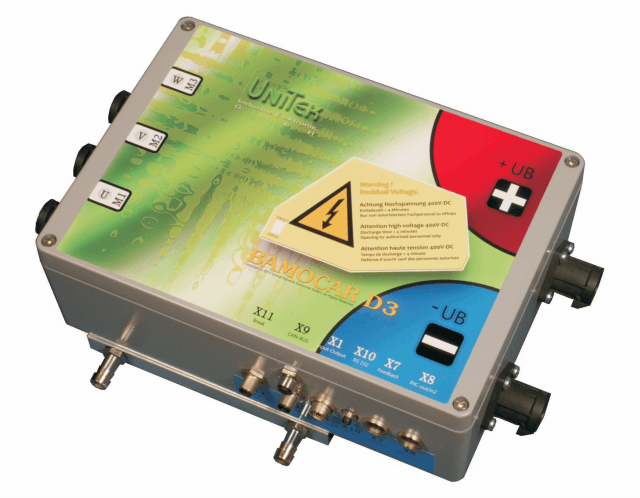
\includegraphics[width=\linewidth]{images/fig17}
        \caption{UniTek Bamocar D3 ESC}
    \end{figure}

    \section{Cooling System}

    The cooling system is designed to be as safe as possible by offering ample cooling, while also making it easy to assemble and maintain. The EMRAX 268 specifies limits to the flow rate and pressure of the cooling loop with a flow rate of 8 litres per minute at 2 bar accounting for vacuum, the loop will be running at 7 litres per minute at 1.5 bar to stay under these limits. The cooling loop (\reffig{fig:cooling-loop}) is a series loop with no parallel lanes, allowing for a simple to install and clean path for a 25/75 glycol/water solution as coolant. The loop will be using multiple temperature and pressure sensors to ensure the coolant will never exceed the pressure or temperature limit of the motor of 2 bar, and motor inlet coolant temperature of \SI{50}{\celsius}. If the 2 bar pressure limit is reached, a solenoid valve will be opened to release some coolant into a release tank, allowing pressure inside the cooling loop to be lowered. In the event of the temperature limit being reached, the motor and controller settings will be lowered to allow for heat to be dissipated from the loop and the temperature to be lowered. A ball valve is also present in order to completely stop the flow of coolant when the power is off and the pod is not running.\\

    \begin{figure}
        \centering
        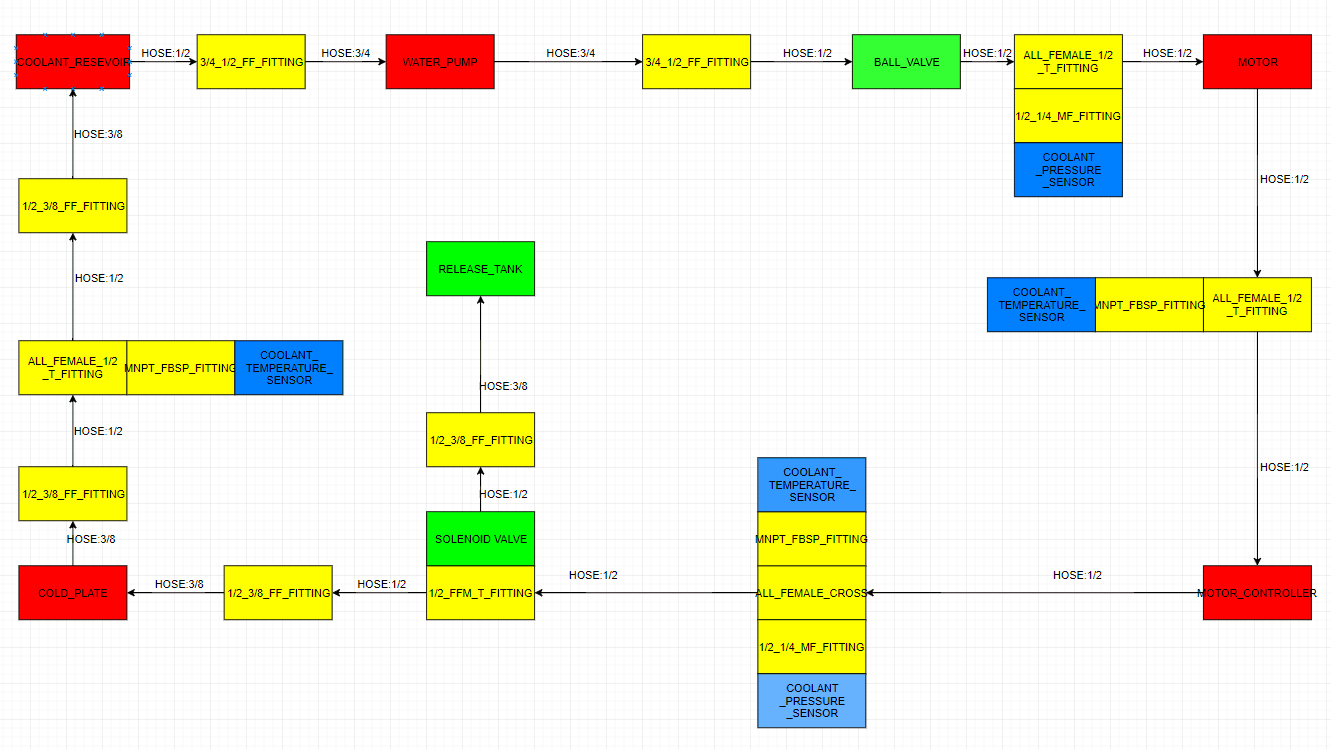
\includegraphics[width=\linewidth]{images/fig18}
        \caption{The cooling loop uses fittings and hoses in order to move from one component to the next seamlessly}
        \label{fig:cooling-loop}
    \end{figure}
    The design parameters of the cooling system used worst-case-scenario heat dissipation numbers: the motor uses \SI{100}{kW} at peak, with specified minimum 92\% efficiency\footnote{EMRAX 268 Technical Data \url{http://emrax.com/wp-content/uploads/2017/01/emrax_268_technical_data_4.5.pdf}}, with the motor controller introducing a maximum of \SI{3}{kW}, so we must dissipate \SI{11}{kW} during a maximum run time of 20 seconds. Using these values and assuming no heat is dissipated through the cold plate and tubing, the total heat input to the loop was calculated using:
\begin{equation}
Q = mC\Delta T
\end{equation}
where $Q$ is \SI{220}{kJ}, $c$ is \SI{3.85}{kJ/kgK} for a 25/75 water/glycol solution at \SI{25}{\celsius}, $m$ is mass of coolant required, and $\Delta T$ is \SI{25}{\celsius}. The mass of coolant required is approximately \SI{2.3}{kg} or $\sim$\SI{2.3}{L}. A 2 litre reservoir was chosen to make up most of the required coolant with the volume of the tubing adding the rest and more. In addition, a cold plate is present in the loop as another safety and redundancy factor in the loop. With the tubing and cold plate dissipating heat, an extra 5 seconds of expected run time, and supplementary coolant mass, it can be estimated that the cooling loop will not exceed a delta temperature of \SI{25}{\celsius}, allowing for a safe acceleration and run of the pod.\\

    The cold plate will be attached to a beam on the ladder frame of the pod, acting as a metal block to absorb any heat that is created. With temperatures not exceeding \SI{50}{\celsius} in the loop before the addition of the coldplate, the aluminum beam will not experience any extreme heat, keeping the integrity of the frame and pod.

    \section{Wheel \& Slip}

    \begin{figure}[H]
        \centering
        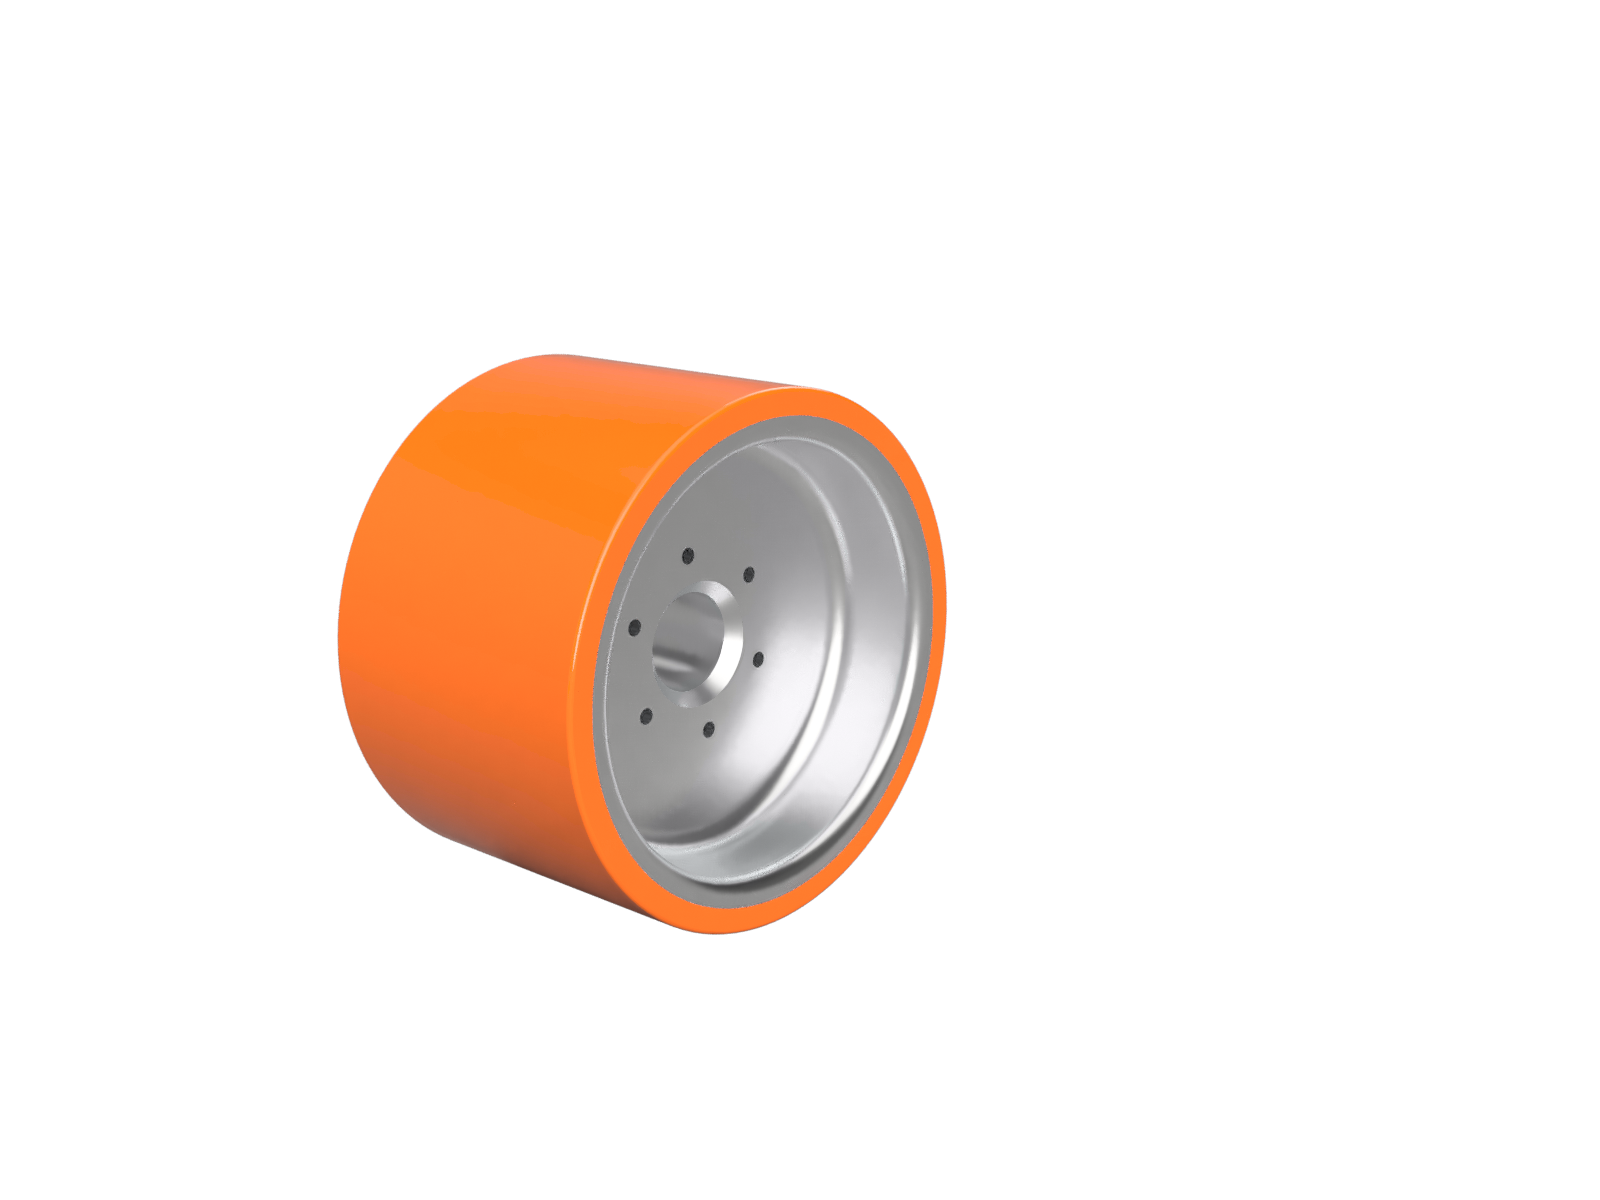
\includegraphics[width=\linewidth]{images/fig19}
        \caption{CAD of Drive Wheel}
    \end{figure}
    Our propulsion system requires strong wheels that are able to withstand high RPM ranges at a large variety of axial and thrust loads. The design was created with an aluminum 6061-T6511 core and a polyurethane wheel tread. Aluminum 6061-T6511 was chosen as the wheel’s core because of the yield strength and low density, as we would require the wheel to be lightweight in order to minimize inefficiency of transferring torque to the ground and the strength such that the wheel will not yield under peak loads. In addition, because this material is easily machined, there is no need for extensive tooling or custom extrusion techniques in order to produce the wheel. 6061-T6511 is a well known and common alloy and thus extensive research has been conducted on the fatigue behaviour of this wheel. Based on fatigue analysis\footnote{\url{https://www.osti.gov/scitech/servlets/purl/10157028}}, even when the wheel has done $10^6$ cycles, it will still be within design specifications and can be used safely.\\

    \subsection{Calculations for slip}
    By using first-principles of Newtonian physics, we can simplify our traction based on static friction. In order to translate angular movement into translational movement, we require that the wheel remain in traction with the track.\\

    Where the overall mass, $m$, of the pod is \SI{150}{kg} and 65\% of the weight is biased towards the drive wheel.

    \begin{center}
        We want to achieve an acceleration of \SI{1}{g} or \SI{9.8}{m/s^2}\\

        Thus, $F_a=m\cdot a = \SI{150}{kg} \times \SI{9.8}{m/s^2} = \SI{1500}{N}$\\

        Frictional force is calculated via $F_f=\mu_s \times F_n$. In this case, $F_f=F_a=\SI{1500}{N}$\\

        Based on the static coefficient of friction of 0.7 with polyurethane vs aluminum,
        \[
        F_n = \frac{F_f}{\mu_s} = \frac{\SI{1500}{N}}{0.7} \approx \SI{2200}{N}
        \]

        But with 65\% biased on the drive wheel, only $\SI{1500}{N} \times 0.6 = \SI{975}{N}$\\

        But we have a deficit in normal force. $\SI{2200}{N} -\SI{975}{N}=\SI{1225}{N}$
    \end{center}
    Based on these calculations, an increase in the normal force between the wheel and the rail was required in order to achieve our nominal acceleration of around 1 g and to prevent slipping of the drive wheel.\\

    The wheel core will be machined from an aluminum billet on a CNC. This will be fairly simple to achieve and does not require any special tooling or machining processes to accomplish. In addition, this allows the balancing of the wheel to be easily achievable due to the lack of manufacturing errors that are produced by casting the wheel. In order to produce the polyurethane tread, we must create a mold and cast the polyurethane tread. This tread will then be chemically secured to the aluminum wheel via vacuum grade epoxy. This process takes the majority of the cost associated with producing the wheel; however, the possibility of machining the tread out of a solid block of polyurethane is currently being investigated as it as a vastly more cost effective solution.

    \begin{figure}[H]
        \centering
        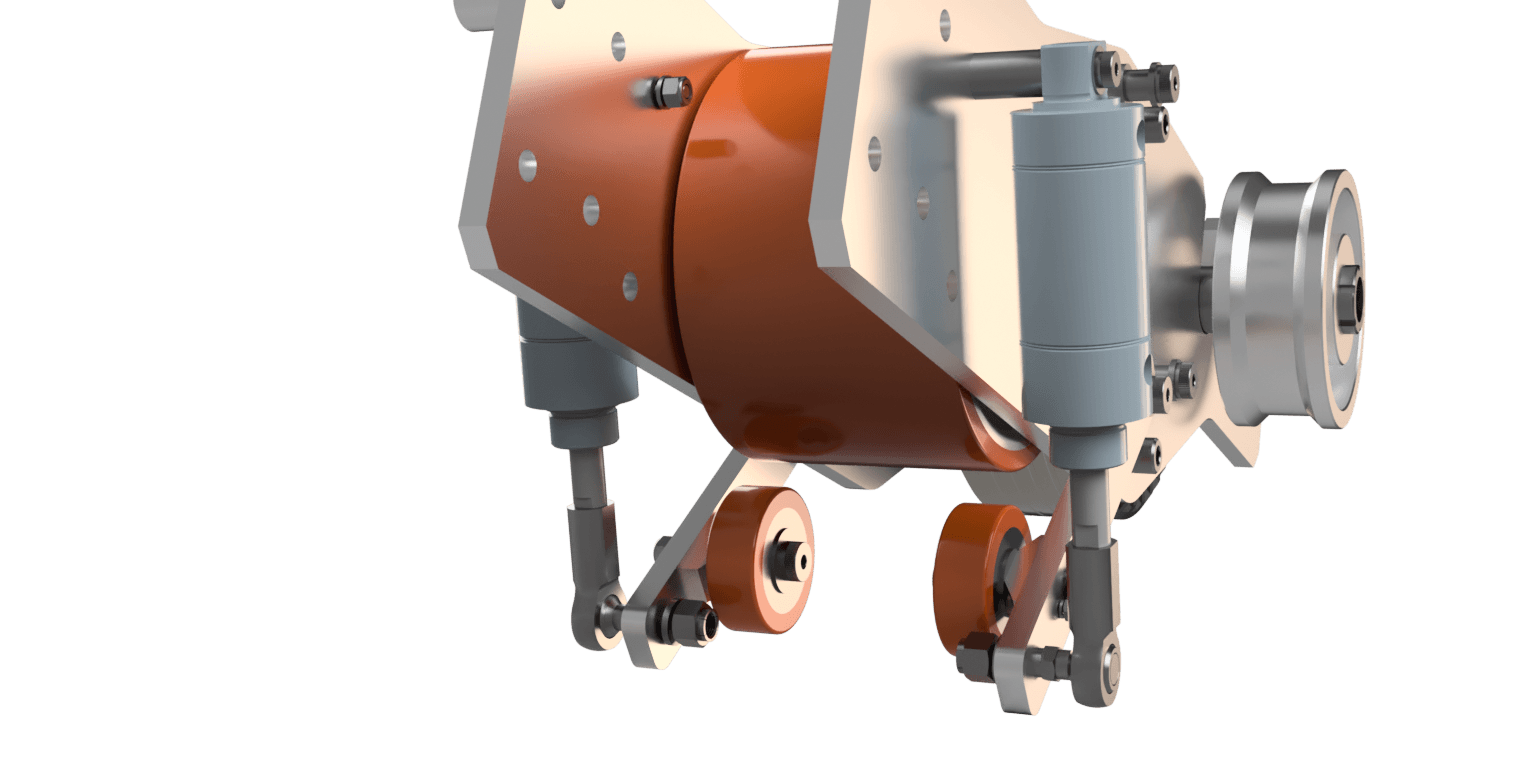
\includegraphics[width=\linewidth]{images/fig20}
        \caption{Pneumatic actuator system mounting to main friction drive structure.}
    \end{figure}
    A solution to our normal force deficit is pneumatic actuators. By utilizing a guide wheel under the I-beam and a pneumatic actuator fastened to a pivot arm to clamp down onto the I-beam flange, we are able to increase the theoretical normal force that the wheel can provide and thus increase our static frictional force. The pneumatic actuator allows us to modulate the traction force needed and dampen any impacts that the guide wheels will encounter while moving down the track.\\

    \section{Pneumatic Circuit}
	The pneumatic circuit provides a damped clamping force for the guide wheels under the I-beam. Using a pneumatic actuator, the retraction and extension of the rod determines the clamping action of the wheels. The retraction of the piston cylinder will move the guide wheels upward to push against the top flange of the I-beam for clamping. In contrast, the extension of the piston cylinder will move the guide wheel downward, releasing the wheels away from the top flange of the I-beam. As calculated earlier, \SI{1400}{N} is provided by the drive wheel. With two guide wheels on either side of drive wheel under the top I-beam flange, \SI{700}{N} is required by each guide wheel for static equilibrium. The pneumatic actuator in the circuit will be a NITRA pneumatic air cylinder with a 2-inch bore diameter. Therefore, the pressurization required for this air cylinder to achieve \SI{700}{N} is calculated as follows:\\

	\begin{center}
		Each piston cylinder has a bore diameter of \SI{2}{in} = \SI{0.0508}{m}\\
        Therefore the bore area is equal to $A = \pi/4 \times {0.0508^2} = \SI{0.00202683}{m^2}$ \\
        To calculate the pressure required:
        \[
      \textrm{Pressure} = \frac{\textrm{Force}}{\textrm{Area}} = \frac{\SI{700}{N}}{\SI{0.00202683}{m^2}} = \SI{50.09}{psi}
        \]
	\end{center}

	Each cylinder must be pressurized \SI{50.09}{psi} on the piston side in order to provide \SI{700}{N} against the wheel. To achieve this, a pressurized tank and pneumatic circuit will be used, as seen in \reffig{fig:pneumatic-diagram} and \reffig{fig:pneumatic-cad}. The tank will contain high pressure air at \SI{3000}{psi}. The high-pressure transmitter will be placed at the tank outlet to provide pressure readings of the tank’s outlet pressure. After the pressure transmitter, a high-pressure relief valve is set to \SI{3000}{psi} to ensure that the high-pressure supply does not exceed the pressure limits of the tank, as well as, the regulator that is placed at the outlet of the PRV. This pressure-reducing regulator will decrease the pressure to \SI{50.09}{psi}. The on/off valve is placed after as a manual fail-safe mechanism. Another pressure transmitter will provide the pressure readings of the low-pressure side of the pneumatic circuit. The pressure relief valve will also be set to \SI{50.09}{psi} to ensure that the pistons are not over-pressurized. The manifold will consist of three tees in order to pressurize the four piston cylinders.  Since the piston cylinders are double-acting, solenoid-operated directional control valves are implemented for each piston. The solenoids will be operated such that the pistons retract to push up the wheels prior to the acceleration phase, and extend to release the wheels after the pod run is complete.\\

	\begin{figure}
        \centering
        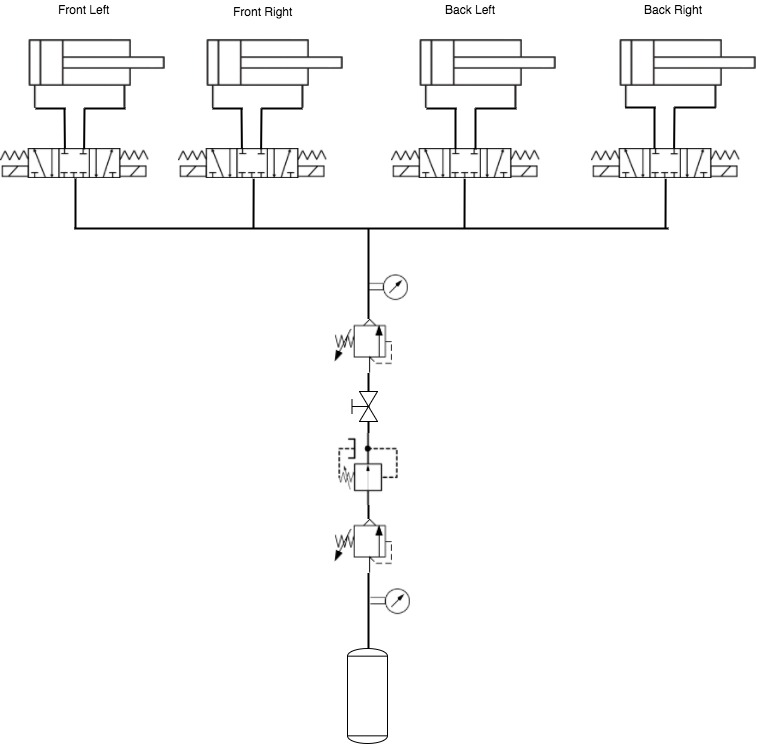
\includegraphics[width=\linewidth] {images/Pneumatic_Circuit}
        \caption{Pneumatic Circuit Schematic Diagram}
        \label{fig:pneumatic-diagram}
    \end{figure}

	\begin{figure}
        \centering
        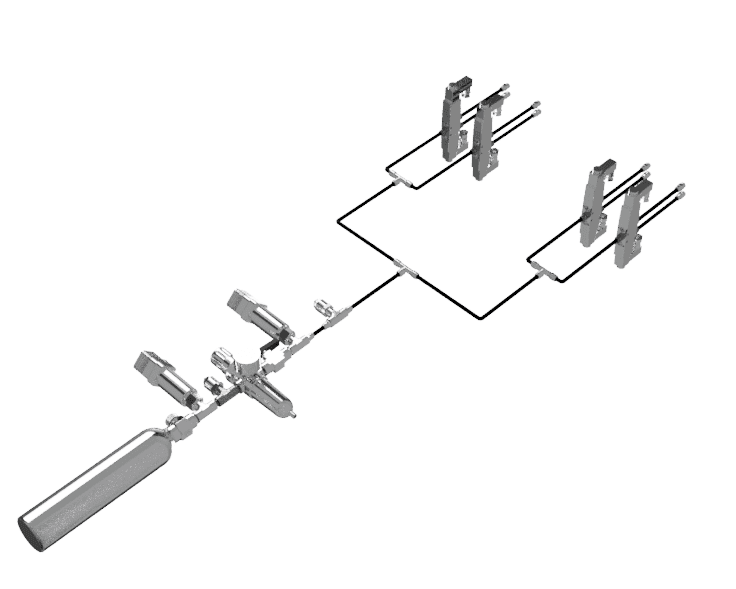
\includegraphics[width=\linewidth] {images/pneumatic_system}
        \caption{CAD of Pneumatic System}
        \label{fig:pneumatic-cad}
    \end{figure}

  \subsection{Mass Flow Choking}
The pneumatic circuit was also designed to ensure that mass flow choking would not be an issue if the regulator fails. To check this condition, the mass flow choking conditions were calculated at the manual on/off valve and the low-pressure relief valve. This was calculated with the mass flow choking equation:\\
\begin{center}
        \[
        {m} = \frac{AP_t}{\sqrt{T_t}} \sqrt{\frac{\gamma}{R}}M(1+\frac{\gamma-1}{2}{M^2})^{-\frac{\gamma+1}{2(\gamma-1)}}
        \]
	\end{center}

The mass flow rate when the flow is choked at the on/off valve was calculated to be \SI{0.409}{kg/s}.
As a result of this relatively high mass flow rate, the \SI{50}{psi} pressure relief valve was designed to a high capacity valve with a mass flow capacity of \SI{0.564}{kg/s}.\\

    \subsection{Pneumatic Circuit Proof Testing}
    In order to certify this pneumatic circuit's MAWP, this system will be hydro-tested at 1.5 MEOP. Since this pneumatic system has a high-pressure side and a low-pressure side, two different MEOP values will be tested. The high-pressure side will be tested to $\SI{800}{psi}\times 1.5=\SI{1200}{psi}$ and the low-pressure side will be tested to $50.09 \times 1.5=75.135$.\\
    The proof testing process will be carried out by filling the system at 1.5 MEOP for 10 minutes. Leaks and pressure gauges will be checked throughout the test to verify the system's functionality.\\

     \subsection{Pneumatic Circuit Explosive Calculations}
     \label{section:pneumatics}
    Explosive calculations were done to check the potential energy of the tank filled with compressed air. To calculate the potential energy of the pneumatic pressure vessel the following equation is used:\\
    \begin{center}
        \[
        U = \frac{P_1 v_1}{k\pm{1}} [1\pm(\frac{P_2}{P_1})^ \frac{k\pm{1}}{k}]
        \]
	\end{center}
	where ${P_1}=\SI{3000}{psia}$, ${P_2}=\SI{14.7}{psia}$, and ${V_1}=\SI{48}{in^3}$, the total energy calculated is \SI{281230.4209}{in}-lb (\SI{31774.77103}{J}) or the  TNT equivalent of \SI{1.44E-02}{lb} (\SI{6.55E-03}{kg}). From this, in can be concluded that this pneumatic system is relatively safe with a line of sight of \SI{37.5}{ft} (\SI{11.4}{m}). However with this calculation, extra precaution will be taken when filling up the tank for safety procedures.

    \subsection{Effects of Pneumatics on Drive Wheel}

    A finite element analysis (\reffig{fig:drive-wheel-stress}) was conducted in Autodesk Fusion 360 by placing a compressive load onto the wheel equivalent to the weight of the pod plus the force that the pneumatic actuators would provide in order to create the required traction force. The track was grounded and fixed in all orthogonal directions and the wheel fixed via the bolt fixtures within the aluminum core.\\

\begin{figure}
        \centering
        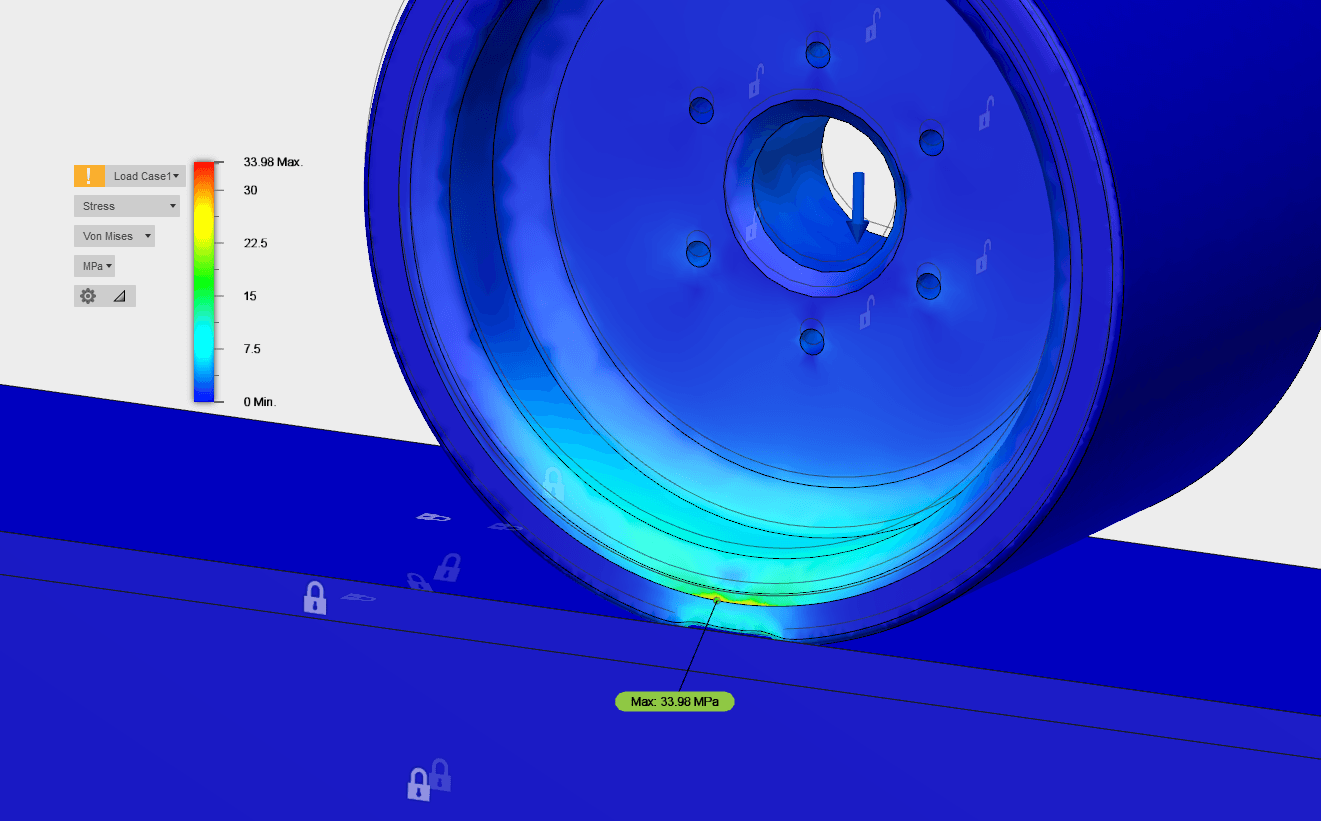
\includegraphics[width=\linewidth]{images/fig21}
        \caption{Static Stress FEA, Peak compressive load on main drive wheel}
        \label{fig:drive-wheel-stress}
    \end{figure}

    At a speed of \SI{100}{m/s}, the aluminum core only experiences a peak stress of \SI{34}{MPa}, which is significantly lower than the yield strength of the material, \SI{275}{MPa}, and provides a safety factor of over 8. At the same speed, the total mass of polyurethane tread, \SI{0.826}{g}, will be subject to 10204 $g$ of radial acceleration, equivalent to \SI{8427}{N} of force.\\

    \begin{center}
    At \SI{100}{m/s}, the outer portion of the \SI{0.2}{m} diameter wheel will experience a radial acceleration as follows:
    	\[
  		\alpha=r\omega^2=\SI{0.2}{m}\times (\SI{100}{rad/s})^2 \times \frac{g}{\SI{9.81}{m/s^2}}= 10204\ g
   		\]
    \end{center}

    The polyurethane tread is a hardness of \SI{90}{A} on the Shore hardness scale. The tensile pressure exerted from the radial acceleration on the tread will be \SI{6.636}{MPa}, lower than the polyurethane's tensile strength of \SI{21.46}{MPa}. The bonding agent between the aluminum wheel and the tread selected is ``3M™ Marine Adhesive Sealant 5200''. This material is rated for above \SI{4.83}{MPa}. More than 40 times higher than the \SI{0.117}{MPa} calculated tensile threshold. Additionally, the bond between the wheel and tread will be subject to \SI{1500}{N} of shear force from the torque generated by the motor. This equates to \SI{0.021}{MPa} of shear stress on the bond. The 3M adhesive is rated for \SI{2.69}{MPa}, giving for a safety factor of 128. \\

    The \SI{0.127}{m} wide and \SI{0.01}{m} thick tread has a cross-sectional area of \SI{0.00127}{m^2}.\\
    This is used to calculate the tensile stress on the tread.
    	\[
  		\textrm{Stress}=\frac{F}{A_{\textrm{cross section}}}=\frac{\SI{8427}{N}}{\SI{0.00127}{m^2}} \times 10^{-6}=\SI{6.636}{MPa}
   		\]
    The surface of contact between the aluminum core and the polyurethane tread is \SI{0.0718}{m^2}.\\
    Thus, the tensile pressure of the adhesive can be calculated:
    	\[
        P_{\textrm{tensile}}=\frac{F}{A_{\textrm{contact}}}=\frac{\SI{8427}{N}}{\SI{0.0718}{m^2}} \times 10^{-6}=\SI{0.1173}{MPa}
        \]
    The torque exerted on the driveshaft will be \SI{135}{Nm}.\\
    By finding the shear force acting between the two components of the wheel, we calculate the shear force the bond must withstand.
    	\begin{gather*}
        F_{\textrm{shear}}=\frac{\tau_{\textrm{drive}}}{r}=\frac{\SI{135}{Nm}}{\SI{0.09}{m}}=\SI{1500}{N}\\
        P_{\textrm{shear}}=\frac{F_{\textrm{shear}}}{A_{\textrm{contact}}}=\frac{\SI{1500}{N}}{\SI{0.0718}{m^2}}=\SI{0.0209}{MPa}
        \end{gather*}
    \begin{figure}
        \centering
        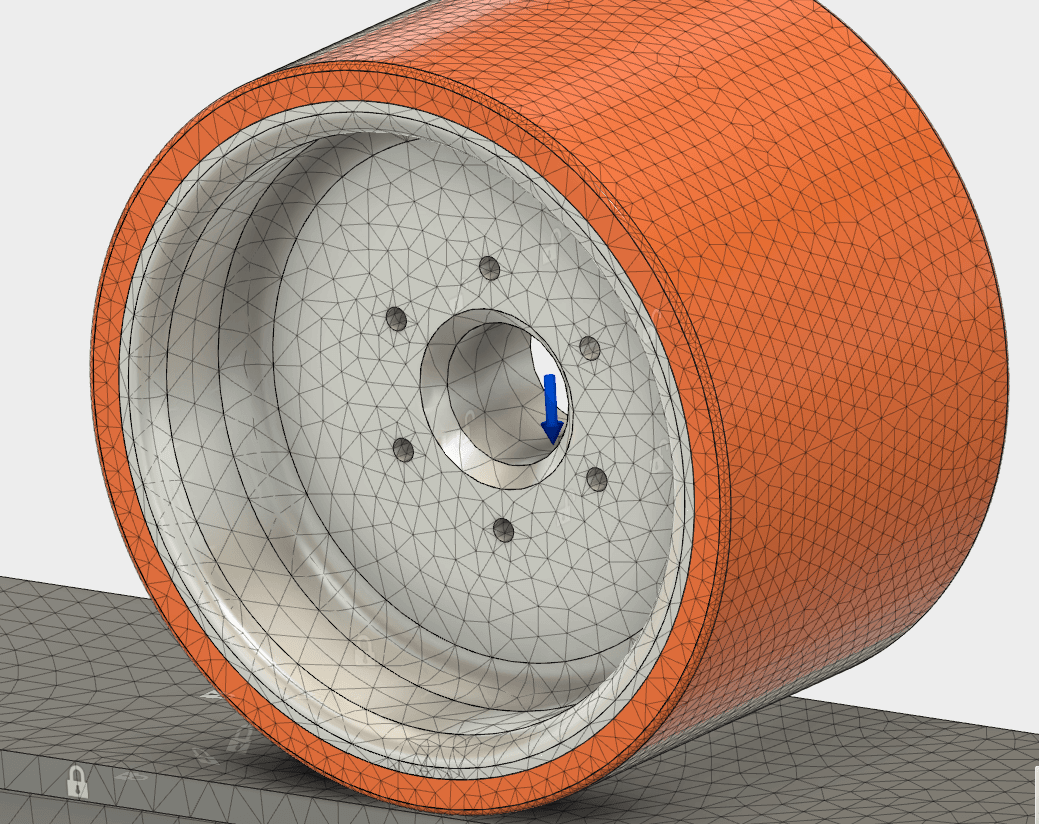
\includegraphics[width=\linewidth]{images/fig22}
        \caption{Caption needed}
        \label{fig:mesh}
    \end{figure}
    The mesh (\reffig{fig:mesh}) was created with an average element size of 2\% \textbf{units?} of the model based size had a parabolic element order. To refine our mesh and create more accurate results, adaptive mesh refinement was done in the areas of peak stress, at a cycle of 6 mesh refinements with a convergence tolerance of 5\%.

    \section{Friction Braking Calipers}
    \label{sec:friction-braking-calipers}
    \begin{figure}[H]
        \centering
        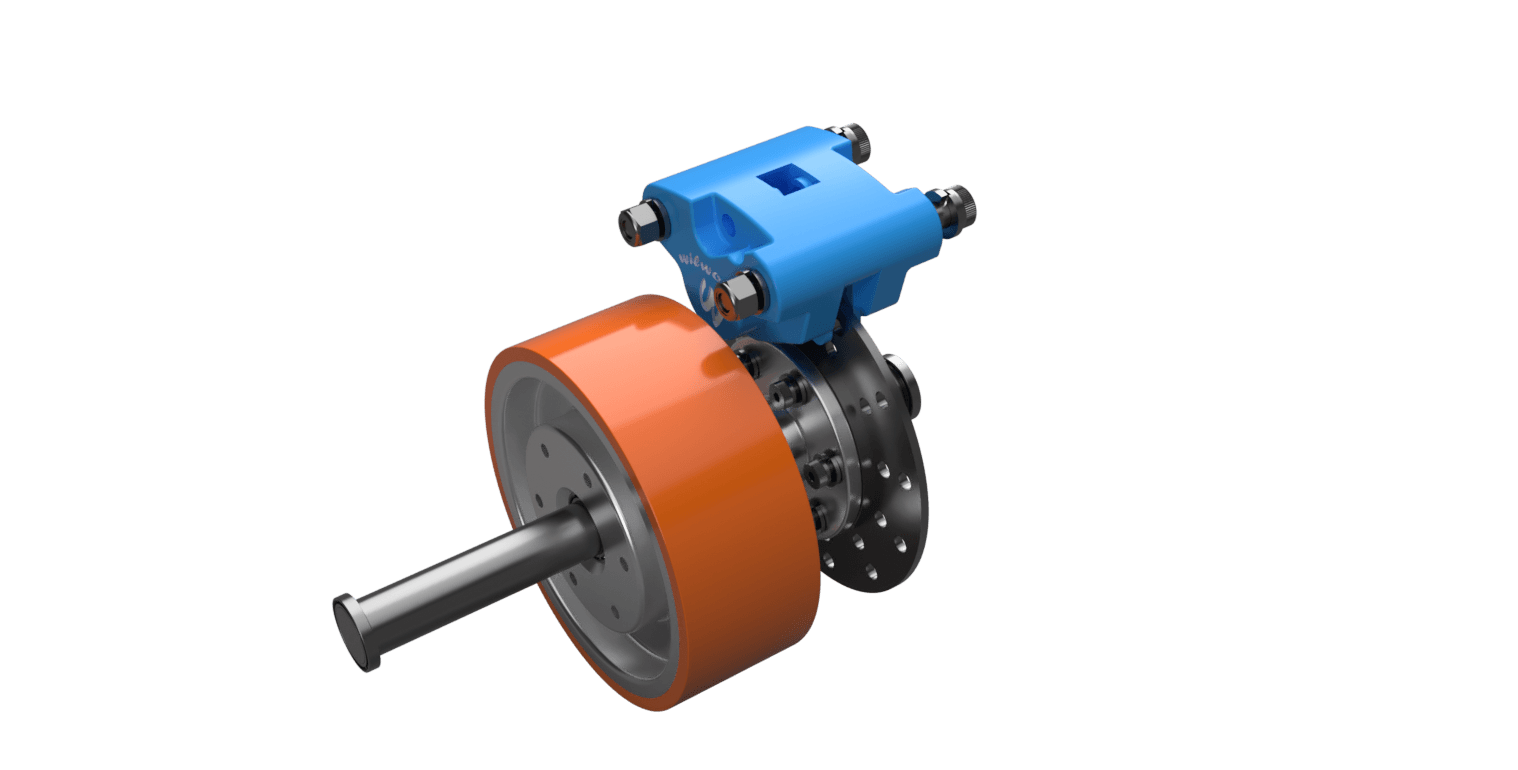
\includegraphics[width=\linewidth]{images/fig23}
        \caption{Caliper design for friction brakes}
    \end{figure}

    \subsection{Motivation}
    Due to Eddy Current Brakes (\refsec{ch:eddy-current-brakes}) being ineffective at speeds below \SI{5}{m/s}, the pod required a secondary braking source to bring it to a complete stop. Friction brake calipers were determined to be the most simple and effective solution, with many off-the-shelf components available. The brakes are not required to perform at high speeds, and as such, do not require large brake rotors or high performance calipers/pads in order to stop the vehicle  As such, there is no requirement to create a custom braking system and the cost associated with creating such a braking system are minimal. It is easily integrated into the original design, requiring little to no alteration to major drivetrain components.\\

    \subsection{Heating}
    The kinetic energy before friction brake is activated is approximately given by:\\
    \[
    	\textrm{Translational kinetic energy} \left(\frac{1}{2}mv^2\right) =\frac{1}{2}(150)(10)^2=\SI{7500}{J}
    \]
    \begin{align*}
	\textrm{Rotational kinetic energy} \left(\sum\frac{1}{2}I{\omega}^2\right)&=\sum\frac{1}{4}mv^2 \\
    &= \frac{1}{4}(5.069)(10)^2 + 4\left(\frac{1}{4}(0.409)(10)^2\right) + \frac{1}{4}(1.209)(10)^2\\
    &= \SI{197.85}{J}
    \end{align*}
    \[
    	\textrm{Total kinetic energy} = \SI{7500}{J} + \SI{197.85}{J} = \SI{7697.85}{J}
    \]

    When the friction brake is activated, kinetic energy will be converted to heat, which will be transferred to the brake rotor disc and the brake pad.\\

    Although the manufacturer did not specifically state the material composition, grey cast iron is the most common material for brake rotor discs. Based on the elemental composition of grey cast iron, the specific heat capacity of the brake disc can be estimated to be \SI{0.465}{J/(g\celsius)} and the mass to be 303.6 g.\\

    Although the brake pad uses sintered metallic material, the material composition is kept confidential by the manufacturer. The composition is drastically different between manufacturers, thus it is rather hard to make an appropriate estimation. Some of the common primary materials are graphite, copper and iron. Carbon steel serves as a decent balance among the three materials, and thus is used to make an approximation.\\

    The density of carbon steel is \SI{0.00785}{g/mm^3}, with a specific heat capacity of \SI{0.49}{J/(g\celsius)}. The volume of the brake pad is \SI{5572}{mm^3}, which approximates the mass to be \SI{43.7}{g}.

    Using the heat transfer equation of $\Delta Q = mc \Delta T$,

    \begin{equation}
    	T=\frac{7697.85}{303.6 \times 0.465+43.7 \times 0.49}=\SI{47.3}{\celsius}
    \end{equation}

    The brake rotor disc and the brake pad will gain approximately \SI{7697.85}{J} of energy, and the temperature will increase by \SI{47.3}{\celsius}.\\

    \subsection{Failsafes}
    The solenoid that controls the brake master cylinder will be on an electrically failsafe circuit. In case of power loss, there will be a reserve battery to make sure that the calipers are actuated at the correct speeds. In addition, these brakes are mechanically failsafe. In the case of complete electrical power loss, the solenoid holding the calipers opens will be a normally open valve and will automatically actuate.
    

    \section{Tests \& Validation (completed and planned)}
	The overall purpose of testing is to verify that the friction drive will be able to function as per design intent. This involves examining certain critical components that may have failure modes that will be detrimental to the functionality of the pod, on or off the track. Testing will also be done to validate certain principles that will be vital to ensuring that the function as per design intent. Some values or concepts are hard to obtain numerically or theoretically, and require empirical testing in order to obtain. Testing will also reveal flaws in design, and will allow us to fix these flaws, in order to be prepared and safe before we enter the competition.\\
    
    Three different testings will be done:
    \begin{itemize}
        \item Motor dynamometer
        \item Wheel endurance testing
        \item Vibration testing
    \end{itemize}

   \begin{figure}
		\centering
       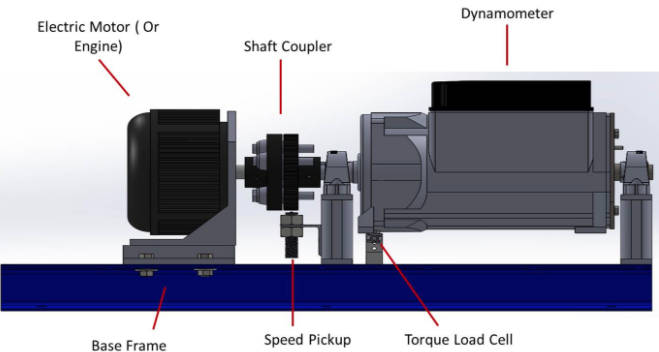
\includegraphics[width=0.5\linewidth]{images/motordyna}
       \caption{Motor Dynamometer}
       \label{fig:motordyna}
   \end{figure}
    A test needs to be conducted with a motor dynamometer (\reffig{fig:motordyna}) to obtain empirical values on motor performance in terms of:
    
    \begin{itemize}
        \item torque/power
        \item RPM ranges
        \item heat generation and thermal profile
        \item power draw (voltage and current)
        \item ESC functionality
        \item power delivery efficiency
    \end{itemize}
    
    Motor performance will be improved by analyzing power/torque curves and optimizing ESC control in order to create a custom map that fits our gear reduction system and acceleration profile. In addition, it allows us to discover and troubleshoot failure modes creates due to design specifications.\\
    
    Moreover, a test to ensure a sufficient endurance level for the wheels is completed. It is crucial to verify that the wheels are able to handle our loads and RPM ranges. A tread wear analysis would be done during acceleration profile and braking phase. A vibration analysis will also be completed to testify that the wheels are two plane balanced.\\

    Furthermore, a vibration test (\reffig{fig:vibra}) will be conducted to test the damping and spring performance and characteristics of the system. This allows us to obtain empirical values of the pod acceleration and position. The analysis provides us with the needed information to tune the suspension to achieve critical damping, and to discover and troubleshoot suspension failure modes.\\

     \begin{figure}
           \centering
       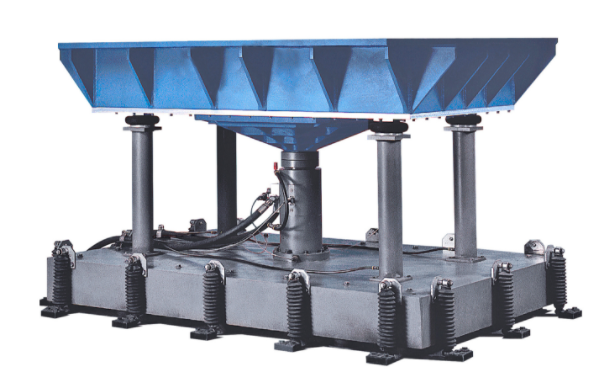
\includegraphics[width=0.5\linewidth]{images/vibra}
       \caption{Vibration testing}
       \label{fig:vibra}
   \end{figure}
    
    \subsection{Flywheel Test Rig}
    We do not yet have detailed design for the flywheel test rig, but it is currently underway. We expect the rig to be completed approximately at the same time as subsystems are completed and assembled.
    
	The main test rig involves a flywheel that comes into contact with the drive wheel, which is used to substitute the I-Beam track, in order to test the endurance of the wheel. This rig can also be used to test eddy current braking and lateral systems.\\
    
    Unfortunately, initial investigation revealed that a full speed test (~90m/s) would require an unreasonably large and strong flywheel, which would be extremely expensive and dangerous to design. Therefore, the current design of the test rig is intended to conduct half-speed tests (~45m/s). This provides a cheaper and more realistic design while still obtaining valuable real-world data from which we can test hypotheses and extrapolate useful conclusions.\\
    
    The flywheel is composed of \SI{16}{in} diameter aluminum bar stock, which replicates the material of the I-Beam, along with additional \SI{12}{in} diameter cast iron bar stock that is used to increase the moment of inertia to the required level. The cost of the flywheel and the mount is approximately 1120 CAD in total. The concept design of the test rig is shown in \reffig{fig:testrig}.\\
    
    \begin{figure}
           \centering
   \begin{subfigure}{0.4\textwidth}
       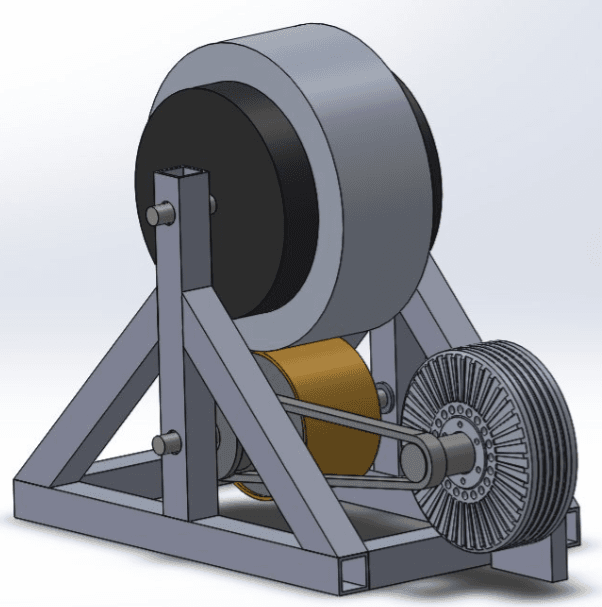
\includegraphics[width=\linewidth]{images/testrig1}
       \caption{}
       \label{fig:testrig1}
       \end{subfigure}        
       \begin{subfigure}{0.4\textwidth}
       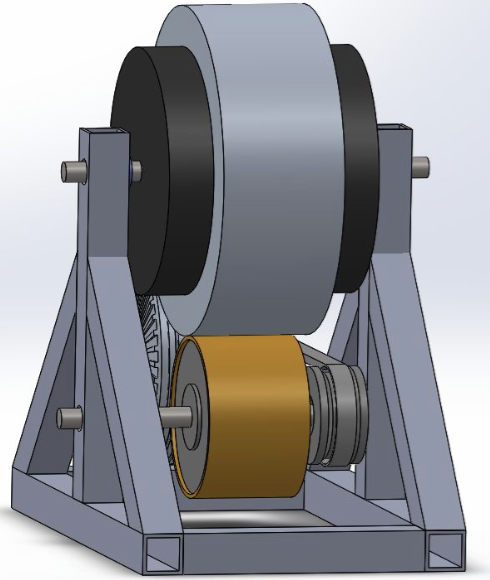
\includegraphics[width=\linewidth]{images/testrig2}
       \caption{}
       \label{fig:testrig2}
       \end{subfigure}
       \caption{CAD views of conceptual test rig design}
       \label{fig:testrig}
   \end{figure}
    
	Since the test rig involves rotating heavy materials at high rotational velocities, safety is critical. A thick protective barrier will be built around the test rig to prevent accidents, such as wheels getting dislodged. In case of emergency, a band brake can be applied to the shaft, which is a simple and reliable solution for braking.\\

\end{document}
